% ------------------------------------------------------------------------------
\documentclass[12pt,t,graphics]{beamer}

% Pacotes ----------------------------------------------------------------------
%\usepackage[brazilian]{babel}
\usepackage[utf8]{inputenc}
\usepackage[T1]{fontenc}
%\usepackage[charter]{mathdesign}                           
\usepackage[font=scriptsize,labelfont=scriptsize]{caption} 
\usepackage{hyperref}
\usepackage{listings}
\usepackage{xcolor}
\usepackage{verbatim}
\usepackage{amsmath}
\usepackage{array,booktabs,tabularx}
\usepackage{alltt}
\usepackage{bibentry}
\usepackage{graphicx}
%\usepackage{multirow}
%\usepackage{textpos}
%\usepackage{appendixnumberbeamer}
\nobibliography*

% Novos comandos ---------------------------------------------------------------
\newcommand{\ds}{\displaystyle}
\newcommand{\vp}{\\\vspace{0.2cm}}
\newcommand{\DIV}[1]{\text{Div}(#1)}
\newcommand{\Div}[1]{\text{div}(#1)}
\newcommand{\Det}[1]{\text{det}(#1)}
\newcommand{\Grad}[1]{\text{grad}(#1)}
\newcommand{\GRAD}[1]{\text{Grad}(#1)}
\newcommand{\DP}[2]{\displaystyle\frac{\partial #1}{\partial #2}}
\newcommand{\bs}[1]{\boldsymbol{#1}}
\newcommand{\bv}[1]{\mathbf{#1}}
\renewcommand{\b}[1]{\boldsymbol{\mathit{#1}}}
\newcommand{\todo}[1]{\textcolor{red}{\textbf{TO DO:} #1}\\}
\newcommand{\ft}[1]{\frametitle{#1}}
\newcommand{\fs}[1]{\framesubtitle{#1}}
\newcommand{\hi}[1]{\textcolor{hilight}{#1}}
\newcommand{\bi}{\begin{itemize}}
  \newcommand{\ei}{\end{itemize}}
\newcommand{\be}{\begin{enumerate}}
  \newcommand{\ee}{\end{enumerate}}
\newcommand{\figw}[2]{\centerline{\includegraphics[width=#2\textwidth]{#1}}}
\newcommand{\figh}[2]{\centerline{\includegraphics[height=#2\textheight]{#1}}}
\newcommand{\fig}[1]{\centerline{\includegraphics{#1}}}
\newcommand{\foot}[1]{\footnotetext{#1}} 

% Default fixed font does not support bold face
\DeclareFixedFont{\ttb}{T1}{txtt}{bx}{n}{12} % for bold
\DeclareFixedFont{\ttm}{T1}{txtt}{m}{n}{12}  % for normal

\makeatletter
\newcommand{\srcsize}{\@setfontsize{\srcsize}{10pt}{10pt}}
\makeatother

% Custom colors
\usepackage{color}
\definecolor{deepblue}{rgb}{0.8,0.4,0}
\definecolor{deepred}{rgb}{0.6,0,0}
\definecolor{deepgreen}{rgb}{0,0.5,0}

% Python style for highlighting

\newcommand\pythonstyle{\lstset{
    language=Python,
    basicstyle=\srcsize\ttfamily,
    otherkeywords={self},             % Add keywords here
    keywordstyle=\ttfamily\color{deepblue},
    % emph={MyClass,__init__},          % Custom highlighting
    emphstyle=\tiny\ttfamily\color{deepred},    % Custom highlighting style
    stringstyle=\color{deepgreen},
    frame=lines,                         % Any extra options here
    linewidth=0.95\textwidth,
    xleftmargin=.05\textwidth,
    showstringspaces=false            % 
  }}


% Python environment
\lstnewenvironment{python}[1][]
{
  \pythonstyle
  \lstset{#1}
}
{}

% Python for external files
\newcommand\pythonexternal[2][]{{
    \pythonstyle
    \lstinputlisting[#1]{#2}}}

% Python for inline
\newcommand\pythoninline[1]{{\pythonstyle\lstinline!#1!}}

% Section page -----------------------------------------------------------------

\captionsetup[figure]{labelformat=empty}

\defbeamertemplate{section page}{mine}[1][]{%
  \begin{centering}
    {\usebeamerfont{section name}\usebeamercolor[fg]{section name}#1}
    \vskip1em\par
    \begin{beamercolorbox}[sep=12pt,center]{part title}
      \usebeamerfont{section title}\insertsection\par
    \end{beamercolorbox}
  \end{centering}
}

\defbeamertemplate{subsection page}{mine}[1][]{%
  \begin{centering}
    {\usebeamerfont{subsection name}\usebeamercolor[fg]{subsection name}#1}
    \vskip1em\par
    \begin{beamercolorbox}[sep=8pt,center,#1]{part title}
      \usebeamerfont{subsection title}\insertsubsection\par
    \end{beamercolorbox}
  \end{centering}
}

\setbeamertemplate{section page}[mine]
\setbeamertemplate{subsection page}[mine]

% Beamer settings --------------------------------------------------------------

\setbeamersize{text margin left=8pt,text margin right=5pt}
\setbeameroption{hide notes}
\setbeamertemplate{note page}[plain]
\usefonttheme{professionalfonts}
\usefonttheme[mathsans/mathserif]{serif}

\usetheme{default}
\beamertemplatenavigationsymbolsempty
\hypersetup{pdfpagemode=UseNone} % don't show bookmarks on initial view

% named colors
\definecolor{offwhite}{RGB}{249,242,215}
\definecolor{foreground}{RGB}{255,255,255}
\definecolor{background}{RGB}{24,24,24}% light
\definecolor{title}{RGB}{107,174,214}
\definecolor{gray}{RGB}{155,155,155}
\definecolor{subtitle}{RGB}{102,255,204}
\definecolor{hilight}{RGB}{102,255,204}
\definecolor{vhilight}{RGB}{255,111,207}
\definecolor{lolight}{RGB}{155,155,155}
\definecolor{myred}{RGB}{232,68,68}

% use those colors
\setbeamercolor{titlelike}{fg=title}
\setbeamercolor{subtitle}{fg=subtitle}
\setbeamercolor{institute}{fg=gray}
\setbeamercolor{normal text}{fg=foreground,bg=background}
\setbeamercolor{item}{fg=foreground} % color of bullets
\setbeamercolor{subitem}{fg=gray}
\setbeamercolor{itemize/enumerate subbody}{fg=gray}
\setbeamertemplate{itemize subitem}{{\textendash}}
\setbeamerfont{itemize/enumerate subbody}{size=\footnotesize}
\setbeamerfont{itemize/enumerate subitem}{size=\footnotesize}
\setbeamerfont{footnote}{size=\tiny}

% page number
\setbeamertemplate{footline}{%
  \raisebox{5pt}{\makebox[\paperwidth]{\hfill\makebox[20pt]{\color{gray}
        \scriptsize\insertframenumber}}}\hspace*{5pt}}

% add a bit of space at the top of the notes page
\addtobeamertemplate{note page}{\setlength{\parskip}{12pt}}

% frametitle
\setbeamertemplate{frametitle}
{
  \nointerlineskip
  \begin{beamercolorbox}[ht=1.8em,wd=\paperwidth]{frametitle}
    \vbox{}
    \insertframetitle\\
    \usebeamerfont{framesubtitle}\quad\insertframesubtitle\strut
    \hfill
    \raisebox{1.6mm}{  %imagem
    }
  \end{beamercolorbox}
  \vspace{-0.3cm}
}

% Para gerar um slide com o titulo da secao
% \AtBeginSection{\frame{\sectionpage}}
% ------------------------------------------------------------------------------

% Title page -------------------------------------------------------------------
\author{
  Lucas Arantes Berg\\
  Programa de Pós Graduação em Modelagem Computacional \\
  UFJF\\
  \texttt{berg@ice.ufjf.br}}

\title{Introdução à Programação com Python}
\subtitle{Semana da Computação - UFJF - 2018}
\institute{}
\date{}

\titlegraphic{
  \centering
  \vspace{-1cm}
  % \includegraphics[scale=0.6]{logo_lncc}
}
% ------------------------------------------------------------------------------

\begin{document}

% ------------------------------------------------------------------------------

\begin{frame}[t,plain]
  \titlepage
\end{frame}


% ------------------------------------------------------------------------------

\frame{\ft{Conteúdo}
  \bi
\item Parte I
  \bi
\item Introdução e Motivação
\item Sintaxe
\item Tipos de Dados
\item Construções básicas (if, while, for)
\item Listas, Tuplas
\item Funções
  \ei
\item Parte II
  \bi
\item Dicionário
\item Orientação a Objetos
\item Programação Funcional
  \ei
\item Parte III
  \bi
\item Computação científica com Python
  \ei
\item Parte IV
  \bi
\item Bibliotecas e programas interessantes
  \ei
  \ei
}

% ------------------------------------------------------------------------------

\begin{frame}
  \title{Parte I}
  \subtitle{Introdução à linguagem Python}
  \date{}\author{}\institute{}\date{}
  \maketitle
\end{frame}

% ------------------------------------------------------------------------------

\frame{\ft{Sobre a linguagem Python}
  \bi
\item Criada por Guido van Rossum em 1991
\item Linguagem de Alto Nível
\item Interpretada
\item Programação:
  \bi
\item Modular
\item Orientada a objetos
\item Funcional
  \ei
\item Tipagem dinâmica e forte
\item Vasta coleção de bibliotecas
\item Código aberto (GPL)
  \ei
}

% ------------------------------------------------------------------------------

\frame{\ft{Sobre a linguagem Python}
  \bi
\item Diversas estruturas de dados nativas
  \bi
\item lista, tupla, dicionário
  \ei
\item Gerenciamento de memória automático
\item Tratamento de exceções
\item Sobrecarga de operadores
\item Indentação para estrutura de bloco
\item Multiplataforma
\item Bem documentada
\item Muito usada
\item Quem usa?
  \bi
\item Blender, GIMP, Inkscape, YouTube, NASA, CERN
\item SPSS, ESRI, ArcGIS, Abaqus, OpenOffice
\item Google, YouTube
\item Battlefield 2, The Sims 4, Civilization IV, Overwatch
  \ei
  \ei
}

% ------------------------------------------------------------------------------

\frame{\ft{Porque usar Python?}
  \bi
\item Fácil, simples
\item Sintaxe limpa
\item Diversas bibliotecas já inclusas
\item Mais expressiva do que muitas linguagens (C/C++,
  Perl, Java)
\item Interativa
\item Protótipos rápidos
\item Alta produtividade
\item Interfaces para outras linguagens como C/C++ e Fortran
  \ei
}

% ------------------------------------------------------------------------------

\begin{frame}[fragile]
  \ft{Vamos começar}
  \bi
\item Python é uma linguagem interpretada
\item Não existe uma etapa de compilação do código, como em C/C++, Fortran
\item Você simplesmente executa o comando python e pode começar a executar código de forma	interativa
  \ei
  \begin{python}
    berg@machine:~/Desktop\$ python
    Python 2.7.15 (default, May 16 2018, 17:50:09) 
    [GCC 8.1.1 20180502 (Red Hat 8.1.1-1)] on linux2
    Type help, copyright, credits ...
    >>>

    >>> print 2 + 2
    4

    >>> print ' pink' + ' floyd'
    pinkfloyd

    >>> x = 2**3	
  \end{python}
\end{frame}

% ------------------------------------------------------------------------------

\begin{frame}[fragile]
  \ft{Alguns detalhes}
  \bi
\item Não é preciso terminar comandos com ;
\item Não é preciso declarar o tipo de dado das	variáveis
  \ei
  \begin{python}
    >>> a = 2**3
    >>> a
    8

    >>> x = 2.9 + 6.5 + 1.1
    >>> x
    10.5

    >>> print type(a)
    <type ' int' >
    >>> print type(x)
    <type ' float'>		
  \end{python}
  \bi
\item Podemos executar códigos: 
  \bi
\item de forma interativa usando o interpretador
  python, como no exemplo acima
\item ou através da linha de comando (fazer uma demonstração):
  
  \item \$ python programa.py 
  \ei
  \ei
\end{frame}

% ------------------------------------------------------------------------------

\begin{frame}[fragile]
  \ft{Tipos de dados}
  \bi
\item Tipos de dados básicos: \pythoninline{int, long, float,	complex, bool}
\item O tipo de uma variável muda conforme o valor	atribuído
  \ei
  \begin{python}
    >>> x / 2
    4
    >>> type(x)
    int
    >>> x = 10.5
    >>> type(x)
    float
    >>> m = (6.8 + 9.4 + 8.4)/3
    >>> m
    8.200000000000001
    >>> m > 6.0
    True
    >>> (m >= 9.0) and (m <= 10.0)
    False
    >>> c1 = 3 + 1j
    >>> c2 = complex(-3,2)
    >>> c1 + c2
    3j		
  \end{python}	
\end{frame}

% ------------------------------------------------------------------------------

\begin{frame}[fragile]
  \ft{Tipos de dados - \texttt{bool}}	
  \bi
\item Tipo de dados \pythoninline{bool}
\item Valores: \pythoninline{True}, \pythoninline{False} e \pythoninline{None}
\item Operadores: \pythoninline{is}, \pythoninline{not}, \pythoninline{and}, \pythoninline{or}
  \ei
  \begin{python}
    >>> x = 11
    >>> x > 0
    True
    >>> x % 2 == 0
    False
    >>> y = True
    >>> not y
    False
    >>> x is not None
    True		
  \end{python}
\end{frame}

% ------------------------------------------------------------------------------

\begin{frame}[fragile]
  \ft{Tipagem forte}
  \begin{python}
    >>> c = "5"
    >>> q = 4
    >>> print c, q
    5 4
    >>> print c + q

    Traceback (most recent call last):
    File "<stdin>", line 1, in <module>
    TypeError: cannot concatenate 'str' and 'int' 
  \end{python}		
  \bi
\item Isto é, Python é uma linguagem dinâmica, mas com
  tipagem forte, ao contrário de outras linguagens
  como Perl que é dinâmica e com tipagem fraca.
\item Tipagem forte costuma ser a característica que não permite um mesmo dado ser tratado como se fosse de outro tipo.

\item Isto dá mais robustez ao código.
  \ei
\end{frame}

% ------------------------------------------------------------------------------

\begin{frame}[fragile]
  \ft{Strings}
  \bi
\item Python define um tipo de dados nativo para
  strings (\pythoninline{str})
\item Strings podem ser delimitadas por aspas simples,
  dupla ou tripla
  \ei
  \begin{python}
    >>> ' simples'
    ' simples'

    >>> " dupla"
    ' dupla'

    >>> """ tripla"""
    ' tripla'

    >>> """ tripla possui uma propriedade especial: 
    elas ignoram quebra de linha, portanto a string 
    aparece como ela eh escrita"""
    ' tripla possui uma propriedade especial: 
    elas ignoram \n'		
  \end{python}
\end{frame}

% ------------------------------------------------------------------------------

\begin{frame}[fragile]
  \ft{Strings}
  \begin{python}
    >>> print("C:\diretorio\novo\nada.exe")
    C:\diretorio
    ovo
    ada.exe		
  \end{python}
  \bi
\item Como evitar a quebra de linha?
  \ei
  \begin{python}
    print("C:\diretorio\\novo\\nada.exe")		
  \end{python}
  \bi
\item Modos especiais de strings:
  \bi
\item raw string
\item unicode string
  \ei
  \ei
  \begin{python}
    >>> print(r' C:\diretorio\novo\nada. exe' )
    C:\diretorio\novo\nada.exe
    >>> print(u" \u2192" )		
  \end{python}		
\end{frame}

% ------------------------------------------------------------------------------

\begin{frame}[fragile]
  \ft{Strings}
  \bi
\item Strings são imutáveis
  \ei	
  \begin{python}
    >>> " hello" + " world" # concatenacao
    'helloworld'
    >>> s = ' hello'
    >>> s[0] = ' j '

    Traceback (most recent call last):
    File " <stdin>" , line 1, in <module>
    TypeError: ' str' object does not support
    item assignment
    
    >>> sn = 'j' + s[1:]
    >>> sn
    'jello'	
  \end{python}
\end{frame}

% ------------------------------------------------------------------------------

\begin{frame}[fragile]
  \ft{Strings}
  \bi
\item O operador ’+’ não converte automaticamente
  números ou outros tipos em strings. A função
  str() converte valores para sua representação em
  string.
  \ei	
  \begin{python}
    >>> pi = 3.14
    >>> text = 'o valor de pi eh = ' + pi
    Traceback (most recent call last):
    File " <stdin>" , line 1, in <module>
    TypeError: cannot concatenate ' str' and ' float' objects
    >>> text = ' o valor de pi eh = ' + str(pi)		
  \end{python}
  \bi
\item Formatadores especiais
  \ei
  \begin{python}
    >>> text = 'o valor de pi eh = %f' % pi
    >>> print text
    >>> a = 10.2
    >>> i = 100
    >>> s = 'oi'
    >>> text = "float=%f int=%d string=%s" % (a,i,s)	
  \end{python}		
\end{frame}

% ------------------------------------------------------------------------------

\begin{frame}[fragile]
  \ft{Strings}
  \bi
\item Acesso sequencial, em fatias ou direto (índice)
\item Slice: s[start:end]
 \ei	
  \begin{python}
    >>> s = "hello"
    >>> s[0]
    'h'
    >>> s[1:]
    'ello'
    >>> s[1:4]
    'ell'
    >>> s[:]
    'hello'
    >>> s[1:100]
    'ello'
  \end{python}	
\end{frame}

% ------------------------------------------------------------------------------

\begin{frame}[fragile]
  \ft{Strings}
  \bi
\item Strings possuem uma grande variedade de métodos:
  \bi
\item lower, upper, capitalize
\item split, strip, join
\item, find, replace
\item startswith, islower, ...
  \ei
  \ei	
  \begin{python}
    >>> ". ".join("PYTHON IS POWERFUL".lower().split()) + "!!! "
    'python. is. powerful!!! s'		
  \end{python}	
  \bi
\item Passo a passo
  \ei
  \begin{python}
    >>> s = "PYTHON IS POWERFUL"
    >>> s.lower()
    'python is powerful'
    >>> s.lower().split()
    ['python' , 'is' , 'powerful']
    >>> a = s.lower().split()
    >>> " . " .join(a)
    'python. is. powerful'
    >>> " . " .join(a) + " !!! "
    'python. is. powerful!!!' 		
  \end{python}
\end{frame}

% ------------------------------------------------------------------------------

\begin{frame}[fragile]
  \ft{Strings}
  \begin{python}
    # split()
    >>> s = 'monty python and the flying circus'
    >>> print s.split()
    ['monty', 'python', 'and', 'the', 'flying', 'circus'] 
    # count()
    >>> print s.count("th")
    # join()
    >>> s = "em busca do calice sagrado"
    >>> s2 = s.split()
    >>> print " /".join(s2)
    em/busca/do/calice/sagrado		
  \end{python}
  \bi
\item Ainda é possível realizar diversas outras
  operações com strings
  \ei
\end{frame}

% ------------------------------------------------------------------------------

\begin{frame}[fragile]
  \ft{Listas e Tuplas}
  \bi
\item Estruturas de dados nativas: list, tuple
\item Coleções de objetos heterogêneos
\item Crescem até o limite da memória
\item Acesso sequencial, em fatias ou direto
\item Métodos para adicionar, remover, ordenar,
  procurar, contar
\item Listas são mutáveis e tuplas são imutáveis
\item Tuplas não podem ser alteradas depois de criadas
\item Listas são delimitadas por [ e ]
\item Tuplas são delimitadas por ( e )
  \ei
\end{frame}

% ------------------------------------------------------------------------------

\begin{frame}[fragile]
  \ft{Tuplas}
  \bi
\item Uma tupla é uma coleção de objetos separados por
  vírgula
  \ei
  \begin{python}
    >>> primos = (2,3,5,7)
    >>> print primos[0], primos[-1]
    2 7
    >>> t_vazia = ()
    >>> print len(t_vazia)
    0
    >>> u_tupla = ('oi' ,)
    >>> print len(u_tupla)
    1
  \end{python}	
  \bi
\item Para uma tupla com 1 elemento apenas é preciso
  usar \pythoninline{(val,)}
  \ei		
\end{frame}

% ------------------------------------------------------------------------------

\begin{frame}[fragile]
  \ft{Tuplas}
  \bi
\item Pode ter ou não parênteses para delimitar a tupla
\item Tupla aninhada
\item Heterogênea
  \ei
  \begin{python}
    >>> t = 12345, 54321, 'hello!' # ou
    >>> t = (12345,54321, 'hello!' )
    >>> t[0]
    12345
    >>> t
    (12345, 54321, 'hello!' )

    # tuplas podem ser aninhadas
    >>> u = t, (1, 2, 3, 4, 5) 
    >>> u
    ((12345, 54321, 'hello!' ), (1, 2, 3, 4, 5))

    # desempacotar tupla
    >>> x,y,z = t 
    >>> print y
    54321		
  \end{python}	
\end{frame}

% ------------------------------------------------------------------------------

\begin{frame}[fragile]
  \ft{Listas}
  \bi
\item "Arrays flexíveis"
  \ei
  \begin{python}
    >>> a = [ 'spam', 'eggs', 100, 1234]
    >>> a
    [ 'spam', 'eggs', 100, 1234]
    >>> a[0]
    'spam'
    >>> a[3]
    1234
    >>> a[-2]
    100
    >>> a[1:-1]
    [ 'eggs', 100]
    >>> a[:2] + [ 'bacon', 2*2]
    [ 'spam', 'eggs', 'bacon', 4]
    >>> 2*a[:3] + ['Boo!']
    ['spam', 'eggs', 100, 'spam', 'eggs', 100, 'Boo!']		
  \end{python}	
\end{frame}

% ------------------------------------------------------------------------------

\begin{frame}[fragile]
  \ft{Listas - Métodos }
  \begin{python}
    >>> a = range(5)
    >>> print a
    >>> a.append(5)
    >>> print a
    >>> a.insert(0,42)
    >>> print a
    >>> a.reverse()
    >>> print a
    >>> a.sort()
    >>> print a	
  \end{python}	
  \bi
\item Saída
  \begin{scriptsize}
\begin{verbatim}
		[0, 1, 2, 3, 4]
		[0, 1, 2, 3, 4, 5]
		[42, 0, 1, 2, 3, 4, 5]
		[5, 4, 3, 2, 1, 0, 42]
		[0, 1, 2, 3, 4, 5, 42]
		
\end{verbatim}
  \end{scriptsize}	
\item Outros métodos:
  \bi
\item remove(x): remove primeira ocorrência de x
\item index(x): retorna o índice da primeira ocorrência de x na lista
  \ei
  \ei	
\end{frame}

% ------------------------------------------------------------------------------

\begin{frame}[fragile]
  \ft{Listas - Métodos}
  \bi
\item As listas contém ponteiros para objetos que
  residem em algum lugar na memória
  \begin{figure}
    \centering
    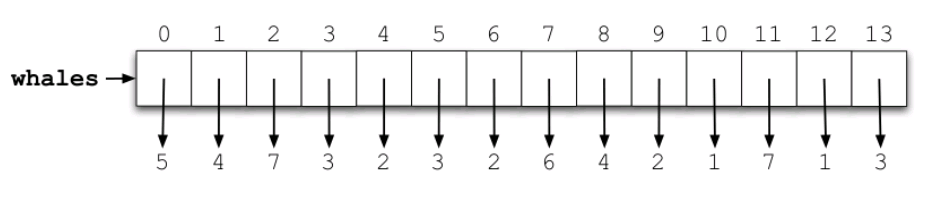
\includegraphics[scale=0.4]{img/lista1.png}
    \label{fig:lista1}
  \end{figure}
\item Alterações
  \begin{figure}
    \centering
    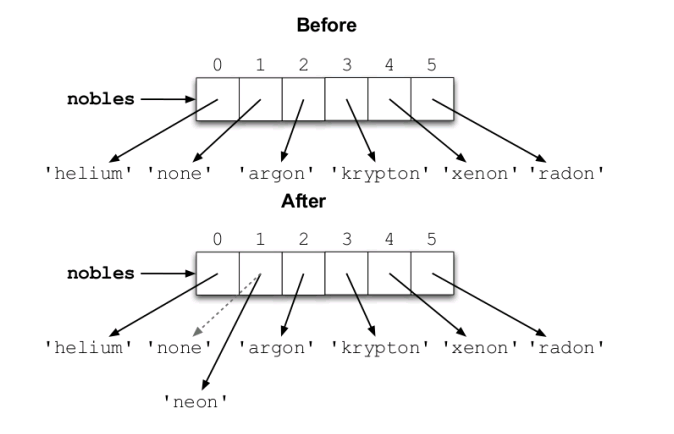
\includegraphics[scale=0.375]{img/lista2.png}
    \label{fig:lista2}
  \end{figure}	
  \ei
\end{frame}

% ------------------------------------------------------------------------------

\begin{frame}[fragile]
  \ft{Listas}
  \bi
\item Concatenação	
  \ei
  \begin{python}
    >>> original = [ 'H', 'He', 'Li' ]
    >>> temp = [ 'Be' ]
    >>> final = original + temp
    >>> print final
    [ 'H', 'He', 'Li', 'Be' ]	
  \end{python}
  \bi
\item Slice
  \ei
  \begin{python}
    >>> l = range(10)
    >>> l[2:6]
    [2, 3, 4, 5]	
  \end{python}	
\end{frame}

% ------------------------------------------------------------------------------

\begin{frame}[fragile]
  \ft{Listas}
  \bi
\item Lista aninhada	
  \ei
  \begin{python}
    >>> la = [['a', 'b'],[1,2],[3,4]]
    >>> print la
    [[ 'a', 'b'], [1, 2], [3, 4]]
    >>> print la[0]
    [ 'a', 'b' ]
    >>> print la[1]
    [1, 2]
    >>> print la[2][1]
    4
  \end{python}
  \begin{figure}
    \centering
    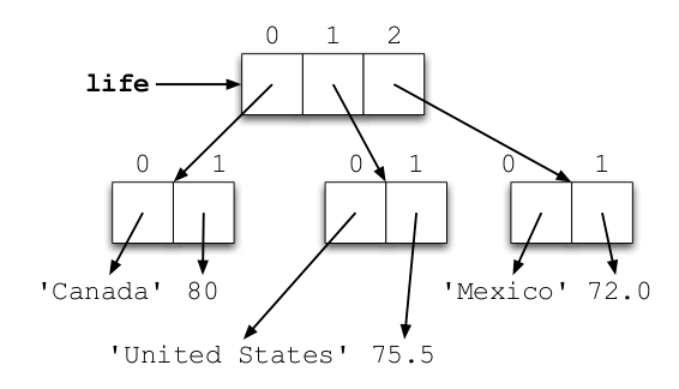
\includegraphics[scale=0.35]{img/lista4.png}
    \label{fig:lista4}
  \end{figure}
\end{frame}

% ------------------------------------------------------------------------------

\begin{frame}[fragile]
  \ft{Built-ins}
  \bi
\item A linguagem Python automaticamente importa
  algumas funções, tipos e símbolos que são
  conhecidos como built-ins.
\item Mecanismos básicos da linguagem.
\item Alguns exemplos
  \bi
\item \pythoninline{range}: para listas
\item \pythoninline{dict}, \pythoninline{list}, \pythoninline{set} e \pythoninline{object} tipos de estrutura de dados
\item \pythoninline{min}, \pythoninline{max} e \pythoninline{sum} para operações matemáticas em listas
\item \pythoninline{help}, \pythoninline{dir}
  \ei
\item Consulte a documentação completa:
  \bi
\item http://docs.python.org/library/functions.html
\item http://docs.python.org/
  \ei
  \ei
\end{frame}

% ------------------------------------------------------------------------------

\begin{frame}[fragile]
  \ft{A função \texttt{range}}
  \bi
\item \pythoninline{help(range)}
  \begin{scriptsize}	
\begin{verbatim}
Help on built-in function range in module __builtin__:

range(...)
   range([start,] stop[, step]) -> list of integers
   
Return a list containing an arithmetic progression of integers.
range(i, j) returns [i, i+1, i+2, ..., j-1]; start (!) defaults to 0.
When step is given, it specifies the increment (or decrement).
For example, range(4) returns [0, 1, 2, 3]. The end point is omitted!
These are exactly the valid indices for a list of 4 elements.	
\end{verbatim}
  \end{scriptsize}	
  \ei
  \begin{python}
    >>> range(10)
    [0, 1, 2, 3, 4, 5, 6, 7, 8, 9]
    >>> range(10,20)
    [10, 11, 12, 13, 14, 15, 16, 17, 18, 19]
    >>> range(10,20,2)
    [10, 12, 14, 16, 18]
    >>> range(20,10,-1)
    [20, 19, 18, 17, 16, 15, 14, 13, 12, 11]		
  \end{python}	
\end{frame}

% ------------------------------------------------------------------------------

\begin{frame}[fragile]
  \ft{Indentação}
  \bi
\item Aviso aos navegantes!
\item Python não usa {; }, begin, end para estrutura de bloco
\item Código em C
  \begin{columns}
    \column{0.4\textwidth}
    \begin{scriptsize}
\begin{verbatim}
if (num % 2 == 0)
{
par = par + 1;
printf("Par");
}
else
{
impar = impar + 1;
printf("Impar");
}	
\end{verbatim}
    \end{scriptsize}
    \column{0.4\textwidth}
    \begin{scriptsize}
\begin{verbatim}
if (num % 2 == 0) {
    par = par + 1;
    printf("Par");
} else {
    impar = impar + 1;
    printf("Impar");
}
\end{verbatim}
    \end{scriptsize}
  \end{columns}
\item Em Python a estrutura de bloco é definida pela
  \textbf{indentação} do código!
  \ei	
\end{frame}

% ------------------------------------------------------------------------------

\begin{frame}[fragile]
  \ft{Indentação}
  \bi
\item Isso mesmo!
\item Tudo que pertence a um mesmo bloco fica alinhado
  no mesmo nível do código fonte.	
  \ei	
  \begin{python}
if num % 2 == 0:
    par = par + 1
    print 'Par'
else:
    impar = impar + 1
    print 'Impar'
  \end{python}
  \bi
\item Erro de indentação
  \ei
  \begin{python}
if x % 2 == 0:
print 'par'

File " <stdin>", line 2
print 'par'
IndentationError: expected an indented block
  \end{python}
\end{frame}

% ------------------------------------------------------------------------------

\begin{frame}[fragile]
  \ft{Estruturas de Controle}
  \bi
\item If-Else
  \ei	
  \begin{python}
if exp:
    comandos
else:
    comandos		
  \end{python}
  \bi
\item If-else-if-else
  \ei
  \begin{python}
if exp:
    comandos
elif exp:
    comandos
else:
    comandos		
  \end{python}	
\end{frame}

% ------------------------------------------------------------------------------

\begin{frame}[fragile]
  \ft{Estruturas de Controle}
  \bi
\item Exemplos
  \ei	
  \begin{python}
>>> x = int( raw_input("Numero: "))
>>> if x < 0:
...     print 'Negativo'
... elif x == 0:
...     print 'Zero'
... else:
...     print 'Positivo'

>>> if ((x >= 0) and (x <= 100)):
...     print "OK"
... else:
...     print "Fora do intervalo"

>>> if ((x<0) or (x>100)):
...     print "Fora do intervalo"
... else:
...     print "OK"		
  \end{python}		
\end{frame}

% ------------------------------------------------------------------------------

\begin{frame}[fragile]
  \ft{Estruturas de Controle}
  \bi
  \item Outras formas de if-else em Python
  \ei	
  \begin{python}
a = 10
b = 20
m = a if(a>b) else b
  \end{python}
  \bi
  \item Equivalente a
  \ei
  \begin{python}
if(a>b):
    m = a
else:
    m = b
  \end{python}
  \bi
  \item Similar ao operador ternário da linguagem C
  \ei
  \begin{python}
m = (a > b) ? a : b;
  \end{python}
\end{frame}

% ------------------------------------------------------------------------------

\begin{frame}[fragile]
  \ft{Estruturas de Controle}
  \fs{For, While}
  \bi
\item \pythoninline{for}
  \ei	
  \begin{python}
lst = [10,20,30, 'oi' , 'ciao' ]
for item in lst:
    print item

for letra in "python":
    print letra
    
for k in range(100):
    print k		
  \end{python}
  \bi
\item \pythoninline{while} sintaxe
  \ei	
  \begin{python}
while exp:
    comandos
    
while exp:
    if exp2:
        comandos1
    comandos2
  \end{python}	
\end{frame}

% ------------------------------------------------------------------------------

\begin{frame}[fragile]
  \ft{Estruturas de Controle}
  \fs{For, While}
  \bi
\item Outro exemplo
  \ei	
  \begin{python}
    >>> a = [ 'cat', 'spider', 'worm' ]
    >>> for x in a:
    ...     print x, len(x)
    ...
    cat 3
    spider 6
    worm 4	
  \end{python}
  \bi
\item De outra forma
  \ei		
  \begin{python}
    >>> for i in range( len(a)):
    ...     print i, a[i]
    ...
    0 cat
    1 spider
    2 worm
  \end{python}	
\end{frame}

% ------------------------------------------------------------------------------

\begin{frame}[fragile]
  \ft{Estruturas de Controle}
  \fs{enumerate()}
  \bi
\item A função \pythoninline{enumerate()} cria pares uteis	
  \ei
  \begin{python}
    >>> nomes = [ 'Ana', 'Maria', 'Carla' ]
    >>> for par in enumerate(nomes):
    ...     print par
    (0, 'Ana' )
    (1, 'Maria' )
    (2, 'Clara' )

    >>> for i,nome in enumerate(nomes):
    ...     print i,nome
    0 Ana
    1 Maria
    2 Clara
  \end{python}	
\end{frame}

% ------------------------------------------------------------------------------

\begin{frame}[fragile]
  \ft{Estruturas de Controle}
  \fs{zip()}
  \bi
\item A função \pythoninline{zip()} recebe um par de sequências como
  entrada e cria uma tupla com os seus elementos
  \ei
  \begin{python}
    >>> nomes = [ 'C.Ronaldo' , 'G.Jesus', 'H.Kane' ]
    >>> gols = [4,0,6]
    >>> for n, g in zip(nomes,gols):
    ...     print '%s fez %d gols' % (n,g)
    ...
    C.Ronaldo fez 4 gols
    G.Jesus fez 0 gols
    H.Kane fez 6 gols
  \end{python}	
\end{frame}

% ------------------------------------------------------------------------------

\begin{frame}[fragile]
  \ft{Estruturas de Controle}
  \fs{Switch}
  \bi
\item Python não possui uma estrutura do tipo switch,
  como C, C++ e Java.
\item Podemos contornar a situação com uma cadeia de
  if-elses
  \ei
  \begin{python}
    >>> if n == 0:
    ...     print 'Voce digitou zero.'
    ... elif n == 1:
    ...     print 'Voce digitou um.'
    ... elif n == 2:
    ...     print 'Voce digitou dois.'
    ... elif n == 3:
    ...     print 'Voce digitou tres.'
    ... else:
    ...     print 'Voce digitou qualquer coisa.'
  \end{python}	
\end{frame}

% ------------------------------------------------------------------------------

\begin{frame}[fragile]
  \ft{Funções}
  \bi
\item Procedimento
  \ei
  \begin{python}
def nome(arg1, arg2, ...):
    comandos
    return
  \end{python}	
  \bi
\item Função
  \ei
  \begin{python}
def nome1(arg1, arg2, ...):
    comandos
    return expressao
    
def nome2(arg1, arg2, ...):
    comandos
    return exp1, exp2, exp3

def nome1(arg1, arg2, argx=valor):
    comandos
    return exp
  \end{python}
\end{frame}

% ------------------------------------------------------------------------------

\begin{frame}[fragile]
  \ft{Funções}
  \bi
\item Exemplos
  \ei
  \begin{python}
>>> def par(n):
...     return (n % 2 == 0)

>>> def fib(n):
...     """ Imprime ate n. """
...     a, b = 0, 1
...     while a < n:
...         print a,
 ...         a, b = b, a+b

>>> par(6) 
True

>>> fib(8) 
0 1 1 2 3 5
  \end{python}	
	\bi
	\item Passagem por referência depende do tipo de objeto
	\item Mutável (Lists)
	\item Imutável (Strings)	
	\ei
\end{frame}

% ------------------------------------------------------------------------------

\begin{frame}[fragile]
  \ft{Funções}
  \bi
\item Podemos criar funções com parâmetros opcionais
  que possuem um valor default pré-definido
  \ei
  \begin{python}
>>> def mult(x, num=2):
...     return x, x*num

>>> a,b = mult(2)
>>> print a,b # 2 4

>>> a,b = mult(2, num=10)
>>> print a,b # 2 20

>>> a,b = mult(3, 5)
>>> print a,b # 3 15
  \end{python}
\end{frame}

% ------------------------------------------------------------------------------

\begin{frame}[fragile]
  \ft{Funções}
  \bi
\item Exemplo
  \ei
  \begin{python}
def divide(a, b):
    """
    Divide operando a e b usando divisao inteira.
    Retorna o quociente e resto da divisao
    em uma tupla.
    """
    q = a / b
    r = a - q * b
    return q, r
  \end{python}
  \bi
\item Uso
  \ei
  \begin{python}
>>> divide(10,2)
(5, 0)
>>> mq, mr = divide(10,3)
>>> print mq, mr
3 1
>>> help(divide)
  \end{python}	
\end{frame}

% ------------------------------------------------------------------------------

\begin{frame}[fragile]
  \ft{\textbf{Hands on}}
  \bi
\item[1.] Escreva uma função que dada uma string que
  representa uma URL de uma página da web, obter
  apenas o endereço da página principal.
\item Exemplo
  \ei
  \begin{python}
url_parse('http://www.facebook.com/fulano/photos')
'www.facebook.com'	
  \end{python}
  \bi
\item[2.] Escreva uma função \pythoninline{somaCumulativa()} que recebe uma
  lista de inteiros como parâmetro e retorna uma lista com a soma cumulativa dos elementos.
  Exemplo:
  \ei
  \begin{center}
    \begin{scriptsize}
    \begin{verbatim}
        l = [1,2,3,4]
        r = somaCumulativa(l)
        print(r)
        [1, 3, 6, 10]
\end{verbatim}
    \end{scriptsize}
  \end{center}
\end{frame}

% ------------------------------------------------------------------------------

\begin{frame}[fragile]
  \ft{\textbf{Hands on}}
 \bi
\item Dicas:
  \bi
\item Crie um arquivo texto \texttt{exercicio1.py} para codificar sua solução.
\item Use o exemplo a seguir como base.
  \ei
  \ei
  \begin{python}
def url_parse(url):
    """
    Implemente a funcao abaixo
    """
    
def main ():
    urlteste = raw_input()
    print url_parse(urlteste)
    
if __name__ == "__main__":
    main()
    
  \end{python}
\end{frame}

% ------------------------------------------------------------------------------

\begin{frame}[fragile]
  \ft{\textbf{Hands on}}
  \bi
\item Módulo
\item Vamos supor que você tenha codificado a função 
  \pythoninline{url\_parse()} em um arquivo fonte chamado \texttt{parser.py}
\item Como posso usar essa função em outros programas?
\item Basta usar os comandos from e import da seguinte
  forma
  \ei
  \begin{python}
from parser import url_parse

a = url_parse("http://www.ufjf.br/deptocomputacao")
print(a)

www.ufjf.br
  \end{python}
\end{frame}

% ------------------------------------------------------------------------------

\begin{frame}
  \title{Parte II}
  \subtitle{Aspectos um pouco mais avançados}
  \date{}\author{}\institute{}\date{}
  \maketitle
\end{frame}

% ------------------------------------------------------------------------------

\begin{frame}[fragile]
  \ft{Dicionário}
  \bi
\item Dicionário é uma estrutura de dados muito útil
  que permite armazenar e recuperar pares de
  chaves-e-valores.
\item Arrays associativos.
\item De forma grosseira podemos dizer que um
  dicionário é uma lista que podemos acessar seus
  elementos através de strings.
  \ei
  \begin{figure}
    \centering
    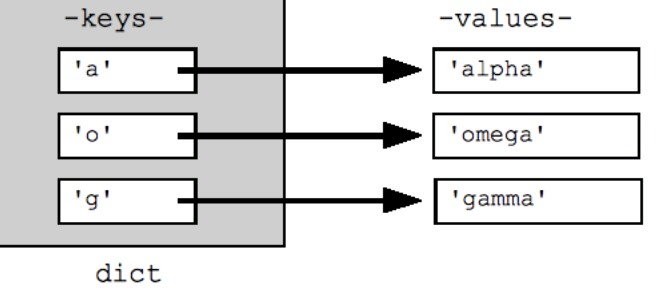
\includegraphics[scale=0.5]{img/dict}
    \label{fig:dict}
  \end{figure}
\end{frame}

% ------------------------------------------------------------------------------

\begin{frame}[fragile]
  \ft{Dicionário}
  \vspace{-0.25cm}
  \begin{python}
>>> d = {}
>>> d[ 'paulo' ] = 25
>>> d[ 'jose' ] = 16
>>> d[ 'alice' ] = 21
>>> print d
{'paulo' : 25, 'jose' : 16, 'alice' : 21}
>>> print d[ 'alice' ]
21
>>> d[ ' alice' ] = 'Paris'
>>> print d
{'paulo' : 25, 'jose' : 16, 'alice' : 'Paris' }
>>> ' jose' in d
True
>>> c = {'MG' : 25.0, 'SP' : 'rain' , 'RJ' : 40.0}
>>> print c[ 'JF' ] # KeyError
>>> if 'JF' in c: print c[ 'JF' ] # evita KeyError
>>> print c.get( 'ES' ) # retorna None
None
>>> novo = dict(a=10, b=20, c=30)
>>> print novo
{'a' : 10, 'c' : 30, 'b' : 20}		
  \end{python}
\end{frame}

% ------------------------------------------------------------------------------

\begin{frame}[fragile]
  \ft{Dicionário}
  \vspace{-0.25cm}
  \bi
\item Percorrendo dicionários
  \ei
  \begin{python}
>>> d = dict(c=10, b=20, a=30)
>>> for key in d:
...     print key

>>> print d.keys()
[ 'a', 'c' , 'b' ]

>>> print d.values()
[30, 10, 20]

# loop sobre as chaves de forma ordenadas
>>> for key in sorted(d.keys()):
...     print key, d[key]

# retorna uma lista onde cada elemento 
# eh uma tupla (chave, valor)
>>> print d.items()
[( 'a', 10), ( 'c', 30), ( 'b', 20)]

>>> for k,v in d.items(): 
...     print k, '->', v		
  \end{python}	
\end{frame}

% ------------------------------------------------------------------------------

\begin{frame}[fragile]
  \ft{List comprehension}
  \bi
\item Como vimos podemos trabalhar com listas
  da seguinte forma
  \ei
  \begin{python}
>>> lista = [2,4,6,8,10]
>>> nova = []
>>> for x in lista:
...     nova.append(x*x)		
  \end{python}
  \bi
\item Entretanto a linguagem Python fornece uma
  sintaxe mais compacta para realizar esse tipo de
  operação.
  \ei
  \begin{python}
>>> nova = [ x*x for x in lista ]
>>> print nova
[4, 16, 36, 64]		
  \end{python}
\end{frame}

% ------------------------------------------------------------------------------

\begin{frame}[fragile]
  \ft{List comprehension}
  \bi
\item Vejamos agora como realizar a seguinte operação
  usando list comprehension
  \ei
  \begin{python}
>>> lista = [2,3,6,7,8,9,10,11]
>>> nova = []
>>> for x in lista:
...     if (x%2)==0:
...         nova.append( str(x))
...
>>> print nova
[ '2', '6', '8', '10' ]
>>>	
  \end{python}
  \bi
\item Podemos reescrever da seguinte forma
  \ei
  \begin{python}
>>> nova = [ str(x) for x in lista if(x%2==0)]		
  \end{python}
  \bi
\item Essa nova versão introduz uma expressão que atua
  como uma espécie de filtro.
\item Muito mais simples e elegante, não?
  \ei	
\end{frame}

% ------------------------------------------------------------------------------

\begin{frame}[fragile]
  \ft{List comprehension}
  \bi
\item Outro exemplo
  \ei
  \begin{python}
>>> txt = "There is someone in my head".split()
>>> nova = [(p.upper(),p.lower(),len(p)) for p in txt]
>>> print nova
[( 'THERE', 'there' , 5),
( 'IS', 'is' , 2),
( 'SOMEONE', 'someone', 7),
...
]	
  \end{python}	
  \bi
\item Lista com todos arquivos .py de um diretório
  \ei
  \begin{python}
>>> import os
>>> from glob import glob
>>> files = [f for f in glob( '*.py' )]
[ 'plotPerfusionCoefs.py', 'findSurf.py' , ...]	
  \end{python}		
\end{frame}

% ------------------------------------------------------------------------------

\begin{frame}[fragile]
   \ft{Classes}
  \bi
\item Vamos apresentar de forma rápida como construir
  classes em Python através de alguns exemplos.
\ei
  \bi
\item Definindo o construtor
  \ei
  \begin{python}
 class Ponto:
    def __init__( self, x, y):
        self.xCoord = x
        self.yCoord = y		
  \end{python}
  \bi
\item Criando um objeto do tipo Ponto
  \ei
  \begin{python}
p = Ponto(2.0, 1.0)
  \end{python}	
\end{frame}

% ------------------------------------------------------------------------------

\begin{frame}[fragile]
  \ft{Classes}
  \bi
\item \pythoninline{self} é um parâmetro especial que precisa ser
  incluído na definição de cada método e precisa
  ser o primeiro parâmetro.
\item Quando um método é invocado, esse parâmetro é
  automaticamente preenchido com a referência ao
  objeto no qual o método foi invocado
  \ei
  \begin{python}
class Ponto:
    def __init__( self, x, y):
        self.xCoord = x
        self.yCoord = y
    
    def getX( self):
        return self.xCoord

    def getY( self):
        return self.yCoord		
  \end{python}
  \begin{python}
p = Ponto(3.0, 1.5)
print p.getX(), p.getY()
  \end{python}
\end{frame}

% ------------------------------------------------------------------------------

\begin{frame}[fragile]
  \ft{Classes}
  \bi
  \item Vamos criar um método para alterar o estado de um \pythoninline{Ponto}
  \ei
  \begin{python}
class Ponto:
    # ...
    def shift(self, xInc, yInc):
        self.xCoord += xInc
        self.yCoord += yInc
  \end{python}
  \bi
  \item Calcular a distância
  \ei
  \begin{python}
class Ponto:
    # ...
    def distancia(self, pt):
        dx = self.xCoord - pt.xCoord
        dy = self.yCoord - pt.yCoord
        return math.sqrt(dx**2 + dy**2)    
  \end{python}
  \bi
  \item Exemplo
  \ei
  \begin{python}
p1 = Ponto(0,0); p2 = Ponto(1.0,1.0)
p2.shift(1.0, 1.0)
print "Distancia = ", p2.distancia(p1)    
  \end{python}
\end{frame}

% ------------------------------------------------------------------------------

\begin{frame}[fragile]
  \ft{Classes}
  \fs{Usando módulos}
  \begin{python}
# Arquivo ponto.py
import math

class Point:
   def __init__( self, x, y ):
       self.xCoord = x
       self.yCoord = y

   def getX( self ):
       return self.xCoord
   
   def getY( self ):
       return self.yCoord

   def shift( self, xInc, yInc ):
       self._xCoord += xInc
       self._yCoord += yInc

   def distance( self, otherPoint ):
       xDiff = self.xCoord - otherPoint.xCoord
       yDiff = self.yCoord - otherPoint.yCoord
       return math.sqrt( xDiff**2 + yDiff**2 )    
  \end{python}
\end{frame}

% ------------------------------------------------------------------------------

\begin{frame}[fragile]
  \ft{Classes}
  \fs{Usando módulos}
  \bi
  \item Podemos usar a classe \pythoninline{Ponto} da seguinte forma:
  \ei
  \begin{python}
from ponto import Ponto

p1 = Ponto(5,7)
p2 = Ponto(0,0)

x = p1.getX()
y = p1.getY()

print( "(" + str(x) + ", " + str(y) + ")" )

p1.shift(4, 12)
d = p1.distancia(p2)  
  \end{python}
\end{frame}

% ------------------------------------------------------------------------------

\begin{frame}[fragile]
  \ft{Classes}
  \fs{Escondendo atributos}
  \bi
  \item Ao contrário da maioria das linguagens que
    suportam orientação a objetos, Python não possui
    um mecanismo para esconder ou proteger os
    atributos de uma classe de acessos externos.
  \item Em C++ temos os modificadores: \texttt{protected, public, private}
  \item O responsável pela classe é que deve indicar
    quais atributos e quais métodos devem ser
    protegidos.
  \item E fica como responsabilidade do usuário da
    classe, não violar essa proteção.
   \item Ainda assim é possível "emular" esse tipo de
    proteção, basta acrescentar dois underlines na
    frente do nome de um atributo ou método.
  \ei
\end{frame}

% ------------------------------------------------------------------------------

\begin{frame}[fragile]
  \ft{Classes}
  \fs{Escondendo atributos}
  \bi
  \item Repare que na implementação anterior da classe
    \pythoninline{Ponto} não protegemos os atributos \pythoninline{xCoord} e
    \pythoninline{yCoord}.
  \item Isso permite que um usuário altere os atributos internos:     
  \ei
  \begin{python}
class Ponto:
    def __init__(self,x,y):
        self.xCoord = x
        self.yCoord = y
  \end{python}
  \begin{python}
>>> p = Ponto(2.0,2.0)
>>> print p.xcoord
2.0

>>> p.xCoord = 'zebra'
>>> print p.xCoord
zebra        
  \end{python}
  \bi
  \item O ideal é que o usuário só altere o estado do
    objeto através de métodos que operem sobre o
    mesmo, e não manipulando os seus atributos.
  \ei
\end{frame}

% ------------------------------------------------------------------------------

\begin{frame}[fragile]
  \ft{Classes}
  \fs{Escondendo atributos}
  \bi
  \item Python permite emular esse ocultamento de informação da seguinte forma:
  \ei
  \begin{python}
class Linha:
  def __init__(self, pA, pB):
    self.__pontoA = pA   # atributo protegido
    self.__pontoB = pB   # atributo protegido

  def pontoA(self):
    return self.__pontoA

  def pontoB(self):
    return self.__pontoB

  def comprimento(self):
    return self.__pontoA.distancia(self.__pontoB)
    
  def mesmoX(self):
    ax = self.__pontoA.getX()
    bx = self.__pontoB.getX()
    return ax == bx
  \end{python} 
\end{frame}

% ------------------------------------------------------------------------------

\begin{frame}[fragile]
  \ft{Classes}
  \fs{Sobrecarga de operadores}
  \bi
  \item Em Python podemos implementar e definir a
    funcionalidade de diversos operadores como \pythoninline{+}, \pythoninline{*}, \pythoninline{==} como parte de nossas classes.
  \ei 
  \begin{python}
class Ponto:
    # ...
    def __eq__(self, outroPonto):
        r = self.xCoord == outroPonto.xCoord and\
            self.yCoord == outroPonto.yCoord
        return r
  \end{python} 
  \bi
  \item Exemplo
  \ei
  \begin{python}
>>> p1 = Ponto(1.0,1.0)
>>> p2 = Ponto(0.0,0.0)
>>> p2.shift(1.0,1.0)
>>> if p1 == p2:
...     print "Os pontos sao iguais."    
  \end{python}
\end{frame}

% ------------------------------------------------------------------------------

\begin{frame}[fragile]
  \ft{Classes}
  \fs{Sobrecarga de operadores}
  \bi
  \item Mais um exemplo
  \ei 
  \begin{python}
class Ponto:
  # ...
  def __str__(self):
      x,y = self.xCoord, self.yCoord
      return " ( %f , %f ) " % (x,y)
  \end{python} 
  \begin{python}
>>> p = Ponto(1.5, 2.5)
>>> print(p)
(1.500000, 1.500000)
  \end{python}
  \begin{figure}
    \centering
    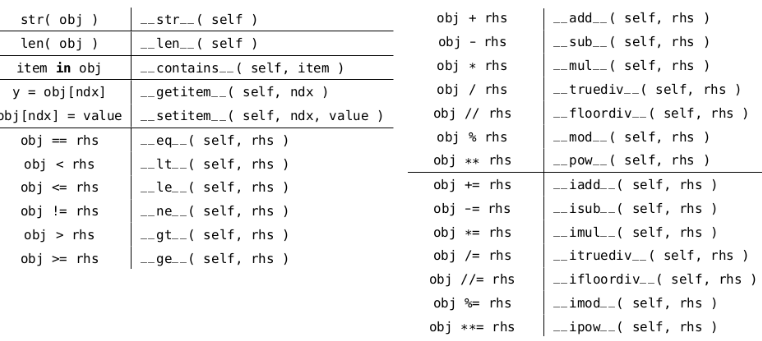
\includegraphics[scale=0.3]{img/ops.png}
  \end{figure}
\end{frame}

% ------------------------------------------------------------------------------

\begin{frame}[fragile]
  \ft{Programação Funcional}
  \bi
  \item Além de suportar programação estruturada e
    orientação a objetos, Python também possui
    recursos de programação funcional.
  \item Vamos apresentar de forma prática alguns destes mecanismos:
    \bi
    \item Funções \pythoninline{lambda}
    \item \pythoninline{map}, \pythoninline{filter} e \pythoninline{reduce}
    \ei
  \item Existem muitos outros recursos de programação
    funcional como iterators e generators, que não
    teremos tempo de discutir.
  \ei 
\end{frame}

% ------------------------------------------------------------------------------

\begin{frame}[fragile]
  \ft{Programação Funcional}
  \fs{map}
  \bi
  \item A função \pythoninline{map} recebe uma sequência (ex: lista) e
    aplica uma função a cada um de seus elementos e
    retorna uma sequência com o resultado da
    aplicação da função.
  \item Calcular o quadrado dos elementos de uma lista
  \ei 
  \begin{python}
>>> def square(num): return num*num
>>> print map(square, range(5))
[0, 1, 4, 9, 16]    
  \end{python}
  \bi
  \item Somar elemento a elemento de duas listas
  \ei
  \begin{python}
>>> def sum(a,b): return a + b
>>> print range(5)
[0, 1, 2, 3, 4]
>>> print range(10,15)
[10, 11, 12, 13, 14]
>>> print map(sum, range(5), range(10,15))
[10, 12, 14, 16, 18]    
  \end{python}
\end{frame}

% ------------------------------------------------------------------------------

\begin{frame}[fragile]
  \ft{Programação Funcional}
  \fs{filter}
  \bi
  \item A função \pythoninline{filter} recebe um predicato e retorna
    apenas os elementos da sequência para os quais o
    predicado resulta no valor \pythoninline{True}.
  \ei 
  \begin{python}
>>> def is_even(num): return num % 2 == 0
>>> print filter(is_even, range(5))
[0, 2, 4]    
  \end{python}

\end{frame}

% ------------------------------------------------------------------------------

\begin{frame}[fragile]
  \ft{Programação Funcional}
  \fs{reduce}
  \bi
  \item A função reduce começa com um valor inicial, e
    reduz a sequência até um único valor aplicando a
    função em cada um dos elementos da sequência
    junto com o valor atual reduzido.
  \item Calcular a soma dos quadrados dos números de 0 a
    4 de uma lista
  \ei
  \begin{python}
>>> def soma(reduced,num): 
...     return reduced + num*num
>>> print reduce(soma, range(5), 0)
30    
  \end{python}
  \bi
  \item Outro exemplo
  \ei
  \begin{python}
>>> a = list([10, 72, 40, 60])
>>> reduce(lambda r,x: x if(x>r) else r, a)   
72
  \end{python}
\end{frame}

% ------------------------------------------------------------------------------

\begin{frame}[fragile]
  \ft{Programação Funcional}
  \bi
  \item Compare com as seguintes versões
  \ei
  \begin{python}
# map
seq = []
for num in range(5):
    seq = seq + [num * num]
print seq

# filter
seq = []
for num in range(5):
    if num % 2 == 0:
        seq = seq + [num]
print seq

# reduce
total = 0
for num in range(5):
    total = total + (num * num)
print total    
  \end{python}
\end{frame}

% ------------------------------------------------------------------------------

\begin{frame}[fragile]
  \ft{Programação Funcional}
  \bi
  \item Python suporta a criação de funções anônimas
    (i.e: funções que não estão ligadas a um nome)
    em tempo de execução, usando uma construção
    através da palavra chave \pythoninline{lambda}.
  \ei 
  \begin{python}
>>> def f (x):
...     return x**2
>>> print f(8)
64

>>> g = lambda x: x**2
>>> print g(8)    
>>> 64
  \end{python}
  \bi
  \item Funções \pythoninline{lambda} não precisam de usar a palavra chave
    \pythoninline{return}
  \ei
\end{frame}

% ------------------------------------------------------------------------------

\begin{frame}[fragile]
  \ft{Programação Funcional}
  \bi
  \item Vejamos um exemplo mais interessante
  \ei 
  \begin{python}
>>> def make_incrementor (n): 
...     return lambda x: x + n

>>> f = make_incrementor(2)
>>> g = make_incrementor(6)

>>> print f(42), g(42)
44 48    
  \end{python}
  \bi
  \item O uso de funções lambda com map, filter e reduce
    é muito prático
  \ei
  \begin{python}
>>> print map(lambda x: x**2, range(5))
[0, 1, 4, 9, 16]

>>> print filter(lambda x: x % 2 == 0, range(5))
[0, 2, 4]

>>> print reduce(lambda r, n: r + n*n, range(5),0)    
30
  \end{python}
\end{frame}

% ------------------------------------------------------------------------------

\begin{frame}[fragile]
  \ft{Programação Funcional}
  \vspace{-0.35cm}
  \bi
  \item \textcolor{red}{Python 3}
  \item Some well-known APIs no longer return lists:
    \bi
    \item map() and filter() return iterators. If you really need a list, a quick fix is e.g. list(map(...)), but a better fix is often to use a list comprehension (especially when the original code uses lambda), or rewriting the code so it doesn’t need a list at all. Particularly tricky is map() invoked for the side effects of the function; the correct transformation is to use a regular for loop (since creating a list would just be wasteful).
    \ei
    \item Builtins
    \bi
    \item Removed reduce(). Use functools.reduce() if you really need it; however, 99 percent of the time an explicit for loop is more readable.
    \ei
  \ei
\end{frame}

% ------------------------------------------------------------------------------

\begin{frame}[fragile]
  \ft{Programação Funcional}
  \bi
  \item No Python 2
  \ei
  \begin{python}
>>> def square(num):
...    return num*num

>>> print map(square, range(5))
[0, 1, 4, 9, 16]
  \end{python}
  \bi
  \item No Python 3
  \ei
  \begin{python}
>>> def square(num):
...    return num*num

>>> print( list(map(square, range(5)) )
[0, 1, 4, 9, 16]   
  \end{python}
\end{frame}

% ------------------------------------------------------------------------------

\begin{frame}[fragile]
  \ft{Arquivos}
  \bi
  \item Arquivos são um tipo built-in do Python que são
  representados por objetos.
  \item Ou seja, não é preciso de importar módulos para
  trabalhar com arquivos em seu programa.
  \item Antes de um arquivo ser usado é preciso primeiro
  criar um objeto que representa o arquivo e então
  abrir o mesmo.
  \ei
  \begin{python}
infile = open('dados.txt', 'r')
outfile = open('notas.txt', 'w')
  \end{python}  	
  \bi
  \item Processamento (lê do arquivo/escreve no arquivo)
  \item Depois que o processamento com os arquivos termina, é preciso
	  fechar os mesmos
  \ei
  \begin{python}
  	infile.close()
  	outfile.close()
  \end{python}    
\end{frame}

% ------------------------------------------------------------------------------

\begin{frame}[fragile]
	\ft{Arquivos}
	\bi
	\item Escrevendo em arquivos
	\ei  
	\begin{python}
ofile = open('notas.txt', 'w')
ofile.write('Notas da Prova\n')
ofile.write(' - ' * 40 + '\n')

for e in estudantes:
    ofile.write('%s \t %6.2f\n' % (e.nome, e.nota))

ofile.write(' - ' * 40 + '\n')
ofile.close()
	\end{python}
	\bi
	\item É preciso colocar explicitamente a quebra de linha \\n no comando 
	\pythoninline{write}, diferentemente do \pythoninline{print}
	\ei
\end{frame}

% ------------------------------------------------------------------------------

\begin{frame}[fragile]
	\ft{Arquivos}
	\bi
	\item Lendo de arquivos
	\ei
	\begin{python}
infile = open("dados.txt", "r")	
line = infile.readline()
data_count = int(line)
for i in range(data_count):
    line = infile.readline()
infile.close()
	\end{python}
	\bi
	\item Podemos usar o metodo \pythoninline{rstrip()} para remover
	espacos em branco à direita
	\ei	
	\begin{python}
line = infile.readline()
sline = line.rstrip()
	\end{python}	
\end{frame}

% ------------------------------------------------------------------------------

\begin{frame}[fragile]
	\ft{Arquivos}
	\bi
	\item Lendo de arquivos
	\ei
	\begin{python}
infile = open("dados.txt", "r")	
line = infile.readline()
data_count = int(line)
for i in range(data_count):
    line = infile.readline()
infile.close()
	\end{python}
	\bi
	\item Podemos usar o metodo \pythoninline{rstrip()} para remover
	espacos em branco à direita
	\ei	
	\begin{python}
		line = infile.readline()
		sline = line.rstrip()
	\end{python}
	\bi
	\item Ou podemos quebrar a linha em várias partes
	\ei
	\begin{python}
# linhas no formato: nome idade nota
line = infile.readline()
temp = line.split()
nome, idade, nota = temp[0], temp[1], temp[2]
	\end{python}	
\end{frame}

% ------------------------------------------------------------------------------

\begin{frame}[fragile]
  \ft{\textbf{Hands on}}
  \bi
  \item[1.] Dada uma lista com palavras (strings), escreva um programa que crie uma lista de inteiros que corresponda ao tamanho das palavras. Escreva duas versões do programa: (i) usando um loop \pythoninline{for} e (ii) usando a função \pythoninline{map()}.
  \item[2.] Escreva uma função \pythoninline{maior_palavra()} que recebe uma lista de palavras e retorna o comprimento da maior palavra da lista. Use apenas as funções \pythoninline{map, filter, reduce} e \pythoninline{lambda} para implementação.
  \ei 
\end{frame}

% ------------------------------------------------------------------------------

\begin{frame}[fragile]
  \ft{\textbf{Hands on}}
  \bi
  \item[3.] Vamos implementar uma função \pythoninline{le\_pontos()} que recebe a string
  com o nome de um arquivo texto, contendo as
  coordenadas de um conjunto de pontos 2D, lê o
  seu conteúdo e retorna uma listas com objetos
  Ponto.
  
  Teremos que usar a classe Ponto definida
  anteriormente.
  
  Exemplo:
  \ei
  \begin{python}
>>> arquivo = "pontos.txt"
>>> pts = le_pontos(arquivo)
>>> for pt in pts:
>   	print pt
(x1,y1) 
(x2,y2)
.
.
.
(xn,yn)   
  \end{python}	
\end{frame}

% ------------------------------------------------------------------------------

\begin{frame}[fragile]
	\ft{\textbf{Hands on}}
	\bi
	\item Considere arquivos de entrada no formato
	\ei
	\begin{python}
9
0.0 0.0
1.0 0.0
2.0 0.0
0.0 1.0
1.0 1.0
2.0 1.0
0.0 2.0
1.0 2.0
2.0 2.0	
	\end{python}	
\end{frame}

% ------------------------------------------------------------------------------

\begin{frame}
  \title{Parte III}
  \subtitle{Computação Científica com Python}
  \date{}\author{}\institute{}\date{}
  \maketitle
\end{frame}

% ------------------------------------------------------------------------------

\begin{frame}[fragile]
  \ft{Workflow Científico}
  \bi
\item Gerar dados (simulação, experimentos)
\item Manipular e processar os dados
\item Visualizar os resultados
  \bi
\item Para entender, interpretar e validar o que
  estamos fazendo
  \ei
\item Comunicar os resultados
  \bi
\item Produzir figuras para relatórios e publicações
\item Apresentações
  \ei
\item Objetivo: apresentar os elementos básicos da
  linguagem Python para escrever programas para
  solução computacional de problemas científicos,
  manipular, processar e visualizar os dados.
  \ei
\end{frame}

% ------------------------------------------------------------------------------

\begin{frame}[fragile]
  \ft{O que é NumPy?}
  \bi
\item Numerical Python
\item Biblioteca para manipulação de arrays
  multidimensionais e matrizes.
\item Operações rápidas em arrays (funções
  vetorizadas)
\item Diferença com relação a listas tradicionais do Python
  \bi
\item Vetor homogêneo
\item Muito mais eficientes do que as listas
\item Número de elemento deve ser conhecido a priori.
\item O array pode ser redimensionado posteriormente.
\item Muito eficiente (implementado em C)
  \ei
  \ei
  \begin{figure}
    \centering
    
\includegraphics[scale=0.4]{img/numpy}
    \label{fig:numpy}
  \end{figure}
\end{frame}

% ------------------------------------------------------------------------------

\begin{frame}[fragile]
  \ft{Python Puro VS NumPy}
  \begin{columns}
  	\column{0.5\textwidth}
	\begin{python}
# Python puro
import time
l = 10000000
start = time.time()

a, b = range(l), range(l)
c = []
for i in a:
    c.append(a[i] * b[i])

t = time.time() - start
print( " Tempo: %s" % t)		
	\end{python}
	Tempo: 2.46 s
  	\column{0.5\textwidth}
	\begin{python}
# NumPy
import time
import numpy as np
l = 10000000
start = time.time()

a = np.arange(l)
b = np.arange(l)
c = a * b

t = time.time() - start
print( " Tempo: %s" % t)		
	\end{python}
	\textbf{Tempo: 0.13 s}
  \end{columns}
\end{frame}

% ------------------------------------------------------------------------------
\begin{frame}[t]{Criando vetores NumPy}
	\begin{itemize}
		\item Arrays NumPy podem ser criados a partir de estruturas de dados do
		Python (listas, tuplas) ou a partir de funções específicas para 
		criação de arrays.
	\end{itemize}
	\begin{scriptsize}
		\begin{table}
			\centering
			\begin{tabular}[c]{|l||l|}
				\hline
				\texttt{zeros((M,N))} & vetor com zeros, M linhas, N colunas \\
				\texttt{ones((M,N))}  & vetor com uns, M linhas, N colunas\\
				\texttt{empty((M,N))} & vetor vazio, M linhas, N colunas\\
				\hline
				\texttt{zeros\_like(A)} & vetor com zeros, mesmo formato de A\\
				\texttt{ones\_like(A)}  & vetor com uns, mesmo formato de A\\
				\texttt{empty\_like(A)} & vetor vazio, mesmo formato de A\\
				\hline
				\texttt{random.random((M,N))} & vetor com numeros aleatorios, MxN\\
				\texttt{identity(N)}    & matriz identidade NxN, ponto flutuante\\
				\texttt{array([[1.5,2,3],[4,5,6]])} & cria a partir de lista ou tupla\\ 
				\hline
				\texttt{arange(I, F, P)}   & vetor com inicio I, fim F, passo P\\
				\texttt{linspace(I, F, N)} & vetor com N números de I até F\\
				\hline
			\end{tabular}
		\end{table}
	\end{scriptsize}
	
\end{frame}

% ------------------------------------------------------------------------------
\begin{frame}[t,fragile]{Criando vetores NumPy}
	\begin{python}
>>> import numpy as np

# np.float64
>>> a = np.array( [36.4, 21.6, 15.6, 27.5] )  
>>> a
array([ 36.4,  21.6,  15.6,  27.5])

# np.float64	
>>> az = np.zeros(4)                          
>>> az
array([ 0., 0., 0., 0.])

# np.int32	
>>> a = np.arange(10)                         
>>> a
array([0, 1, 2, 3, 4, 5, 6, 7, 8, 9])

# np.float64	
>>> a = np.arange(0.0, 1.0, 0.2)              
>>> a
array([ 0. ,  0.2,  0.4,  0.6,  0.8])
	\end{python}
\end{frame}

% ------------------------------------------------------------------------------

\begin{frame}[t,fragile]{Criando vetores NumPy}
\begin{python}
>>> a = np.linspace(0.0, 1.0, 6)
>>> print a
[ 0.   0.2  0.4  0.6  0.8  1. ]
>>> print a.size, a.ndim, a.shape    
6 1 (6,)
	
>>> m = a.reshape(2,3)
>>> print m
[[ 0.   0.2  0.4]
[ 0.6  0.8  1. ]]
>>> print m.size, m.ndim, m.shape
6 2 (2, 3)
	
>>> Z = np.zeros((3,3))
>>> print Z
[[ 0.  0.  0.]
[ 0.  0.  0.]
[ 0.  0.  0.]]
\end{python}
\end{frame}

% ------------------------------------------------------------------------------
\begin{frame}[t,fragile]{Acessando arrays}
	\begin{itemize}
		\item Exemplo com array bidimensional
	\end{itemize}
	\begin{columns}
		\column{.8\textwidth}
		\begin{python}
>>> a = np.arange(24)
>>> a = a.reshape((4,6))
>>> a[2,4]
16
		\end{python}
		%\column{.2\textwidth}
		
		%\begin{figure}
		%	\centering
		%	\includegraphics[scale=0.65]{svg/array1.png} 
		%\end{figure}
	\end{columns}
\end{frame}

% ------------------------------------------------------------------------------
\begin{frame}[t,fragile]{Acessando arrays}
	\begin{columns}
		\column{.8\textwidth}
		\begin{python}
>>> a = np.arange(24)
>>> a = a.reshape((4,6))
>>> a[2,4]
16

>>> a[1]
array([ 6,  7,  8,  9, 10, 11])
		\end{python}
%		\column{.2\textwidth}
%		\begin{figure}
%			\centering
%			\includegraphics[scale=0.65]{svg/array2.png}
%		\end{figure}
	\end{columns}
\end{frame}

% ------------------------------------------------------------------------------
\begin{frame}[t,fragile]{Acessando arrays}
	\begin{columns}
		\column{.8\textwidth}
		\begin{python}
>>> a = np.arange(24)
>>> a = a.reshape((4,6))
>>> a[2,4]
16
>>> a[1]
array([ 6,  7,  8,  9, 10, 11])
		
>>> a[-1]
array([18, 19, 20, 21, 22, 23])
		\end{python}
%		\column{.2\textwidth}
%		\begin{figure}
%			\centering
%			\includegraphics[scale=0.65]{svg/array3.png}
%		\end{figure}
	\end{columns}
\end{frame}

% ------------------------------------------------------------------------------
\begin{frame}[t,fragile]{Acessando arrays}
	\begin{columns}
		\column{.8\textwidth}
		\begin{python}
>>> a = np.arange(24)
>>> a = a.reshape((4,6))
>>> a[2,4]
16
>>> a[1]  # ou a[1,:]
array([ 6,  7,  8,  9, 10, 11])
>>> a[-1]
array([18, 19, 20, 21, 22, 23])
		
>>> a[:,1]
array([ 1,  7, 13, 19])
		\end{python}
%		\column{.2\textwidth}
%		\begin{figure}
%			\centering
%			\includegraphics[scale=0.65]{svg/array4.png}
%		\end{figure}
	\end{columns}
\end{frame}

% ------------------------------------------------------------------------------
\begin{frame}[t,fragile]{Acessando arrays}
	\begin{columns}
		\column{.8\textwidth}
		\begin{python}
>>> a = np.arange(24)
>>> a = a.reshape((4,6))
>> a[2,4]
16
>>> a[1]  # ou a[1,:]
array([ 6,  7,  8,  9, 10, 11])
>>> a[-1]
array([18, 19, 20, 21, 22, 23])
>>> a[:,1]
array([ 1,  7, 13, 19])
		
>>> a[1:3,:]
array([[ 6,  7,  8,  9, 10, 11],
[12, 13, 14, 15, 16, 17]])		
		\end{python}
%		\column{.2\textwidth}
%		\begin{figure}
%			\centering
%			\includegraphics[scale=0.65]{svg/array5.png}
%		\end{figure}
	\end{columns}
\end{frame}

% ------------------------------------------------------------------------------
\begin{frame}[t,fragile]{Acessando arrays}
	\vspace{-0.5cm}
	\begin{columns}
		\column{.8\textwidth}
		\begin{python}
>>> a = np.arange(24)
>>> a = a.reshape((4,6))
>>> a[2,4]
16
>>> a[1]  # ou a[1,:]
array([ 6,  7,  8,  9, 10, 11])
>>> a[-1]
array([18, 19, 20, 21, 22, 23])
>>> a[:,1]
array([ 1,  7, 13, 19])
>>> a[1:3,:]
array([[ 6,  7,  8,  9, 10, 11],
	[12, 13, 14, 15, 16, 17]])
		
>>> a[1:4,2:5]
array([[ 8,  9, 10],
	   [14, 15, 16],
	   [20, 21, 22]])
		\end{python}
%		\column{.2\textwidth}
%		\begin{figure}
%			\centering
%			\includegraphics[scale=0.65]{svg/array6.png}
%		\end{figure}
	\end{columns}
\end{frame}

% ------------------------------------------------------------------------------
\begin{frame}[t,fragile]{Acessando arrays}
	\vspace{-0.5cm}
	\begin{columns}
		\column{.8\textwidth}
		\begin{python}
>>> a = np.arange(24)
>>> a = a.reshape((4,6))
>>> a[2,4]
16
>>> a[1]  # ou a[1,:]
array([ 6,  7,  8,  9, 10, 11])
>>> a[-1]
array([18, 19, 20, 21, 22, 23])
>>> a[:,1]
array([ 1,  7, 13, 19])
>>> a[1:3,:]
array([[ 6,  7,  8,  9, 10, 11],
[12, 13, 14, 15, 16, 17]])

>>> a[::2,::3]
array([[ 0,  3],
[12, 15]])
		\end{python}
%		\column{.2\textwidth}
%		\begin{figure}
%			\centering
%			\includegraphics[scale=0.65]{svg/array7.png}
%		\end{figure}
	\end{columns}
\end{frame}

% ------------------------------------------------------------------------------
\begin{frame}[t,fragile]{Operações com arrays}
	\begin{itemize}
		\item NumPy suporta operações aritméticas entre arrays sem o uso de loops
		com \texttt{for} (implementado em C)
		%  \item Para arrays com mesmo \textit{shape} 
	\end{itemize}
	\begin{python}
>>> import numpy as np
>>> a,b = np.arange(1,11), np.arange(1,11)
>>> a
array([ 1, 2, 3, 4, 5, 6, 7, 8, 9, 10])
>>> a + 1
array([ 2, 3, 4, 5, 6, 7, 8, 9, 10, 11])
>>> a * 2
array([ 2, 4, 6, 8, 10, 12, 14, 16, 18, 20])
>>> a * b
array([ 1, 4, 9, 16, 25, 36, 49, 64, 81, 100])
>>> a ** 3
array([ 1, 8, 27, 64, 125, 216, 343, 512, 729, 1000])
	\end{python}
\end{frame}

% ------------------------------------------------------------------------------
\begin{frame}[t,fragile]{Operações com arrays}
	\begin{itemize}
		\item Outras operações
	\end{itemize}
	\begin{python}
	>>> a=np.array([1,0,1])
	>>> b=np.array([2,2,4])
	>>> np.dot(a,b)
	6
	
	>>> a = np.array([1,0,0])
	>>> b = np.array([0,1,0])
	>>> np.cross(a,b)
	array([0, 0, 1])
	
>>> a,b = np.array([1,2,3]), np.array([1,2,3])
>>> np.outer(a,b)
array([[1, 2, 3],
       [2, 4, 6],
       [3, 6, 9]])
	\end{python}
\end{frame}

% ------------------------------------------------------------------------------
\begin{frame}[t,fragile]{Funções e Arrays NumPy}
	\begin{columns}
		\column{.4\textwidth}
		\begin{itemize}
			\item Avaliar funções usando arrays NumPy
			\item Exemplo: $f(x) = e^{\sin(x)}$
			\item Loops em vetores NumPy muito grandes são lentos
			\item Alternativas:
			\begin{itemize}
				\item \textit{Vectorization}
				\item NumPy oferece diversas funções prontas
			\end{itemize}
		\end{itemize}
		\column{.6\textwidth}
		\begin{python}
from math import exp, sin
import numpy as np
		
def f(x):
    return exp(sin(x))
		
x = np.linspace(0.0, 6.0, 100)
y = np.zeros(x.size)
		
for i in range(x.size):
    y[i] =  f(x[i])
		\end{python}
	\end{columns}
\end{frame}

% ------------------------------------------------------------------------------
\begin{frame}[t,fragile]{Vectorization}  
	\vspace{-0.5cm}
	\begin{columns}   
		\column{.4\textwidth}
		\begin{itemize}
			\item Aplicar $f$ diretamente em todo o vetor
			\item Muito mais eficiente
			\item Mais compacto e fácil de ler
			\item Nem todas funções \texttt{def func(x)} estão prontas
			para serem usadas desta forma
		\end{itemize}
		\vspace{-0.5cm}
		\begin{figure}
			\centering
			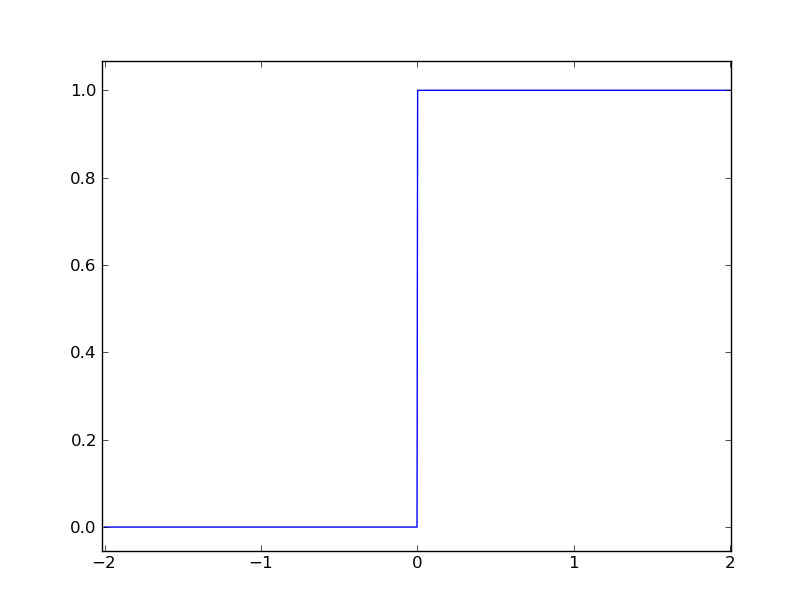
\includegraphics[scale=0.2]{img/hv.png}
		\end{figure}
		\column{.6\textwidth}
		\begin{python}
import numpy as np
		
def f(x):
    return np.exp(np.sin(x))
		
x = np.linspace(0.0, 6.0, 1000)
y = f(x)
\end{python}
		\pause
		\begin{python}
# funcao degrau 
def H(x):
    if (x<0):
    	return 1
    else:
    	return 0
		\end{python}
	\end{columns}
\end{frame}

% ------------------------------------------------------------------------------
\begin{frame}[t,fragile]{Vectorization}
	
	\begin{python}
	>>> x = np.linspace(-1,1,5)
	array([-1. , -0.5, 0. , 0.5, 1. ])
	>>> x < 0
	array([ True, True, False, False, False])
	\end{python}
	
	\begin{itemize}
		\item Como vetorizar funções assim?
		\item Usar a função \pythoninline{where}
		\item Uso: \pythoninline{where(condition, x1, x2)}
		\item Retorna um array do mesmo tamanho de \pythoninline{condition}, onde o 
		elemento \pythoninline{i} é igual a \pythoninline{x1[i]} se \pythoninline{condition[i]} é 
		\pythoninline{True}, ou igual a \pythoninline{x2[i]} caso contrário (\pythoninline{False}).
	\end{itemize}
	
\end{frame}

% ------------------------------------------------------------------------------
\begin{frame}[t,fragile]{Vectorization}
	\begin{itemize}
		\item Forma geral
	\end{itemize}
	\begin{python}
def fun_vec(x):
    cond = <exp_condicao>
    x1 = <expressao1>
    x2 = <expressao2>
    return np.where(cond, x1, x2)
	\end{python}
	\begin{itemize}
		\item Para o exemplo anterior temos
	\end{itemize}
	\begin{python}
def Hv(x):
    cond = x < 0
    return np.where(cond, 0.0, 1.0)
	\end{python}
	
\end{frame}

% ------------------------------------------------------------------------------
\begin{frame}[t,fragile]{Alguns métodos dos vetores}
	\begin{scriptsize}
		\begin{table}
			\centering
			\begin{tabular}[c]{|l||l|}
				\hline
				\texttt{a.sum()} & soma todos elementos \\
				\texttt{a.min()} & menor elemento\\
				\texttt{a.max()} & maior elemento\\
				\texttt{a.mean()}& média aritmética\\
				\texttt{a.std()} & desvio padrão\\
				\texttt{a.var()} & variância\\
				\texttt{a.trace()} & traço\\
				\hline
				\texttt{a.copy()} & retorna cópia\\
				\texttt{a.conjugate()} & complexo conjugado\\ 
				\hline
			\end{tabular}
		\end{table}
	\end{scriptsize}
	
	\begin{python}
	>>> notas = np.array([6., 7.5, 8., 9.2, 4.3])
	>>> notas.mean()
	7.0
	>>> notas.max()
	9.2
	>>> notas.min()
	4.3
	\end{python}
\end{frame}

% ------------------------------------------------------------------------------
\begin{frame}[t,fragile]{Copiando Arrays}
	\begin{itemize}
		\item A expressão $a = x$ faz com que $a$ aponte para 
		o mesmo array que $x$. Logo, mudanças em $a$ também 
		irão afetar $x$
	\end{itemize}
	\begin{python}
	>>> x = np.array([1., 2., 3.5])
	>>> a = x
	>>> a[-1] = 3 # tambem altera x[-1]
	>>> x
	array([1., 2., 3.])
	
	>>> x = np.array([1.,2.,3.5])
	>>> a = x.copy()
	>>> a[-1] = 9
	>>> a
	array([ 1.,  2.,  9.])
	>>> x
	array([ 1. ,  2. ,  3.5])
	\end{python}
\end{frame}

% ------------------------------------------------------------------------------
\begin{frame}[t,fragile]{Matrizes}
	\begin{itemize}
		\item Os arrays usados até então são do tipo \textbf{ndarray}
		\item NumPy também possui um tipo chamado \textbf{matrix}
		\item Sempre bidimensional
		\item Algumas propriedades especiais de matrizes:
		\begin{itemize}
			\item matrix.I (inversa)
			\item matrix.T (transposta)
			\item matrix.H (conjugada)
			\item matrix.A (converte para array)
		\end{itemize}
		\item Operador de multiplicação (*) efetua as operações usuais
		da Álgebra Linear
		\begin{itemize}
			\item matriz-matriz
			\item matriz-vetor
			\item vetor-matriz
		\end{itemize}
	\end{itemize}
\end{frame}

% ------------------------------------------------------------------------------
\begin{frame}[t,fragile]{Matrizes}
	\vspace{-0.25cm}
		\begin{python}
>>> import numpy as np
>>> m=np.matrix([[1, 2], [3,4]])
>>> m
matrix([[1, 2],
        [3, 4]])
>>> m.I
matrix([[-2. ,  1. ],
        [ 1.5, -0.5]])
>>> m.T
matrix([[1, 3],
        [2, 4]])
       
# continua ...             
		\end{python}
\end{frame}

% ------------------------------------------------------------------------------
\begin{frame}[t,fragile]{Matrizes}
	\vspace{-0.25cm}
	\begin{python}	
>>> b = np.array([2,1])
>>> b = np.matrix(b)

>>> b             # vetor linha
matrix([[2, 1]])  

>>> b * m         # vet * mat
matrix([[5, 8]])

>>> b = b.T       # vetor coluna
>>> b
array([[2],
       [1]])
       
>>> m * b         # mat * vet
matrix([[ 4],
        [10]])
        
>>> m * m.I       # mat * mat
matrix([[1.0000e+00, 1.1102e-16],
        [0.0000e+00, 1.0000e+00]])
	\end{python}
\end{frame}

% ------------------------------------------------------------------------------
\begin{frame}[t,fragile]{Matrizes e Álgebra Linear}
	\begin{columns}
		\column{.3\textwidth}
		
		\begin{itemize}
			\item O módulo \textbf{numpy.linalg} possui diversas funções de Álgebra Linear
			\item Solução de Sistema de Equações Lineares
		\end{itemize}
		\begin{align*}
		3x + 2y + 4z &= 1\\
		1x + 1y + 2z &= 2\\
		4x + 3y - 2z &= 3
		\end{align*}
		\column{.7\textwidth}
		\begin{python}
>>> import numpy.linalg as linalg
>>> A = np.matrix([[3.,2.,4.],
                   [1.,1.,2.],
                   [4.,3.,-2.]])
>>> A
matrix([[ 3.,  2.,  4.],
        [ 1.,  1.,  2.],
        [ 4.,  3., -2.]])
>>> b = np.matrix([[1.],[2.],[3.]])
>>> b
matrix([[ 1.],
        [ 2.],
        [ 3.]])
>>> x = linalg.solve(A,b)
>>> x
matrix([[-3.],
        [ 5.],
        [ 0.]])
		\end{python}
	\end{columns}
\end{frame}

% ------------------------------------------------------------------------------
\begin{frame}[t,fragile]{Ajuste de Curvas}
	\begin{columns}
		\column{.5\textwidth}
		\begin{itemize}
			\item Dado os valores de uma função $f(x)$ em um conjunto de pontos,
			encontrar uma função $g(x)$ que melhor se aproxime de $f(x)$.
			\item Aproximação polinomial pelo método dos mínimos quadrados
			\item $g(x) \Rightarrow $ combinação de funções polinomiais
			\item \textbf{numpy.polyfit(x,y,degree)}
		\end{itemize}
		\column{.5\textwidth}
		\begin{figure}
			\centering
			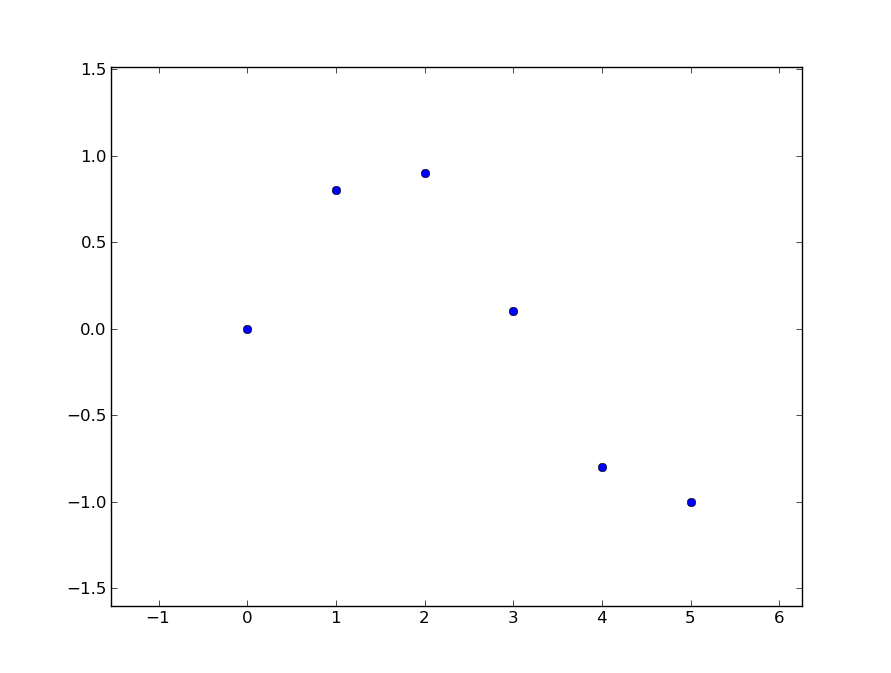
\includegraphics[scale=0.25]{img/ac_dados.png}
		\end{figure}
		\begin{tiny}
			\begin{table}
				\centering
				\begin{tabular}[c]{|l||cccccc|}
					\hline
					$x$ & 0.0 & 1.0& 2.0& 3.0& 4.0& 5.0 \\
					\hline
					$f(x)$ & 0.0 & 0.8 & 0.9 & 0.1 & -0.8 & -1.0\\
					\hline
				\end{tabular}
			\end{table}
		\end{tiny}
	\end{columns}
\end{frame}

% ------------------------------------------------------------------------------
\begin{frame}[t,fragile]{Ajuste de Curvas}
	\begin{columns}
		\column{.6\textwidth}
		\vspace{-0.3cm}
		\begin{python}
>>> import numpy as np

>>> x=np.array([0.0, 1.0, 2.0, 
3.0, 4.0, 5.0]) 

>>> y=np.array([0.0, 0.8, 0.9,
0.1, -0.8, -1.0]) 

>>> c1 = np.polyfit(x, y, 1) 
>>> c1
array([-0.30285714,  0.75714286])
>>> p1 = np.poly1d(c1) 

>>> c3 = np.polyfit(x, y, 3) 
>>> c3
array([ 0.08703704, -0.81349206, 
1.69312169, -0.03968254])
>>> p1 = np.poly1d(c3) 
		
		\end{python}
		\column{.4\textwidth}
		\vspace{-1cm}
		\begin{figure}
			\centering
			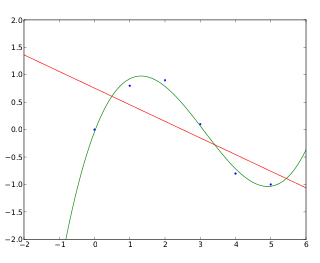
\includegraphics[scale=0.4]{img/ac_deg1deg3.png}
		\end{figure}
	\end{columns}
\end{frame}

% ------------------------------------------------------------------------------
\begin{frame}[t,fragile]{SciPy}
	\begin{itemize}
		\item Coleção de algoritmos matemáticos e funções utilitárias
		\item Implementado em cima do NumPy
		\item Dividido em sub-módulos
		\begin{itemize}
			\item constants: Constantes físicas
			\item fftpack: Transformada Rápida de Fourier
			\item integrate: Integração numérica e ODE solvers
			\item interpolate: Interpolação (Splines)
			\item stats: Distribuições e funções estatísticas
			\item optimize: Otimização
			\item sparse: Matrizes esparsas
			\item linalg: Álgebra Linear
			\item io: Entrada e Saída
			\item signal: Processamendo digital de sinais
			\item ndimage: Processamento digital de imagens
		\end{itemize}
	\end{itemize}
\end{frame}

% ------------------------------------------------------------------------------
\begin{frame}[t,fragile]{Integração Numérica com SciPy}
	\begin{itemize}
		\item Exemplo: $\displaystyle\int_{0}^{4} x^2 \ dx$ 
	\end{itemize}
	\begin{python}
	>>> from scipy import integrate
	>>> def fx2(x):
	>>>     return x*x
	
	>>> integrate.quad(fx2, 0.0, 4.0)
	(21.333333333333332, 2.3684757858670003e-13)
	
	>> print 4.**3/3
	21.3333333333
	\end{python}
	\begin{itemize}
		\item \textbf{integrate.quad} usa um método de quadratura adaptativa
		implementado em Fortran no pacote QUADPACK
	\end{itemize}
	
\end{frame}

% ------------------------------------------------------------------------------
\begin{frame}[t,fragile]{Integração Numérica com SciPy}
	\begin{itemize}
		\item Mais métodos disponíveis
		\begin{itemize}
			\item fixed\_quad: quadratura Gaussiana
			\item odeint: integrar Equações Diferenciais Ordinárias
		\end{itemize}
		\item Integrar dados discretos
		\begin{itemize}
			\item trapz, simps e romb
		\end{itemize}
	\end{itemize}
	\begin{python}
>>> x = linspace(0.0, 4.0, 25)
>>> y = fx2(x)
array([0.0, 0.16667, 0.3333, ..., 4.0])
	
>>> integrate.trapz(y, dx=x[1]-x[0])
21.351851851851851
	\end{python}
\end{frame}

% ------------------------------------------------------------------------------
\begin{frame}[t,fragile]{Visualização de dados com matplotlib}
	\begin{itemize}
		\item A biblioteca matplotlib permite a visualização de dados 2D seguindo o
		estilo do MATLAB
		\item Gráficos de qualidade para publicações
		\item Exporta para diversos formatos
		\item Possibilidade de embutir em interfaces gráficas (Qt, GTK, ...)
		\item Baseado no NumPy e SciPy
		\item \textbf{pylab}: módulo com diversas funções para plotar gráficos 
		de forma fácil
	\end{itemize}
	\begin{figure}
		\centering
		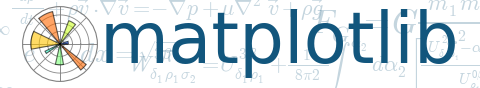
\includegraphics[scale=0.5]{img/matplotlib.png}
	\end{figure}
\end{frame}

% ------------------------------------------------------------------------------
\begin{frame}[t,fragile]{matplotlib}
	\begin{itemize}
		\item Exemplo mais simples de uso: \textbf{plot(x,y)}
		\item Gráficos são gerados sucessivamente, i.e., cada chamada a função
		\textbf{plot} altera o gráfico
	\end{itemize}
	\begin{columns}
		\column{.55\textwidth}
		\begin{python}
>>> import numpy as np
>>> from pylab import *
>>> x = np.linspace(0,3,51)
>>> y = x**2 * np.exp(-x**2)
>>> plot(x,y)
>>> show()
		\end{python}
		\column{.5\textwidth}
		\begin{figure}
			\centering
			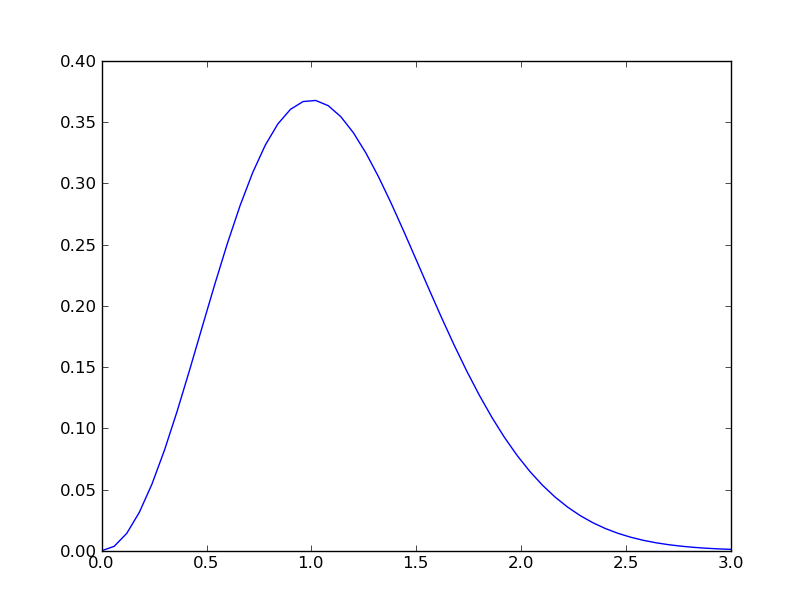
\includegraphics[scale=0.265]{img/plot1.png}
		\end{figure}
	\end{columns}
\end{frame}

% ------------------------------------------------------------------------------
\begin{frame}[t,fragile]{matplotlib}
	\vspace{-0.5cm}
	\begin{itemize}
		\item Decorando o gráfico
	\end{itemize}
		\begin{python}
>>> import numpy as np
>>> from pylab import *
>>> x = np.linspace(0,3,51)
>>> y = x**2 * np.exp(-x**2)
>>> plot(x,y)
>>> grid(True)
>>> xlabel('x')
>>> ylabel('f(x)')
>>> title("Exemplo")
>>> show()
		\end{python}
		\begin{figure}
			\centering
			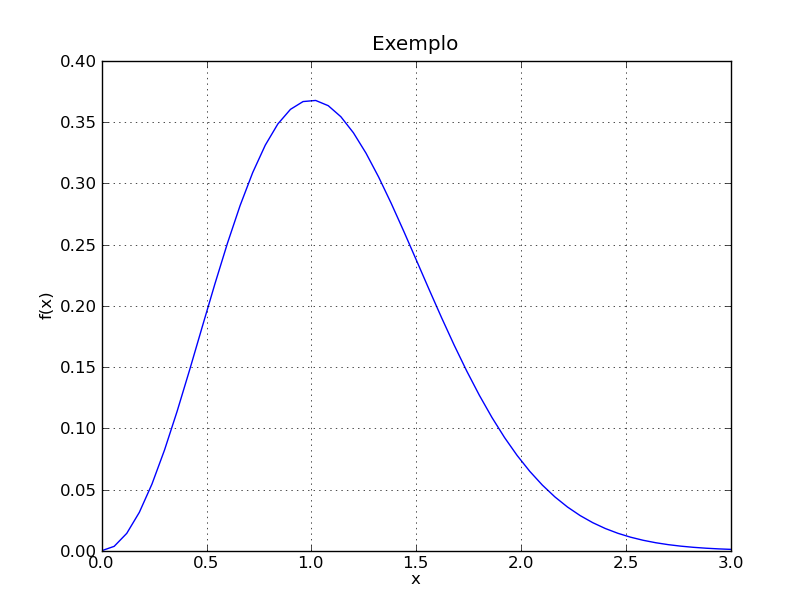
\includegraphics[scale=0.225]{img/plot2.png}
		\end{figure}		
\end{frame}

% ------------------------------------------------------------------------------
\begin{frame}[t,fragile]{matplotlib}
	\vspace{-0.5cm}
	\bi
	\item Várias curvas
	\ei
	\begin{python}
>>> y = np.linspace(-3, 3, 10)
>>> plot(y)
		
>>> x = np.linspace(0, 9, 100)
>>> plot(x,sin(x))
>>> plot(x,cos(x),linestyle='--',color='r')
>>> plot(x,exp(sin(x)),linestyle='-.',color='m')
>>> grid(True)
>>> show()	
		\end{python}
		\begin{figure}
			\centering
			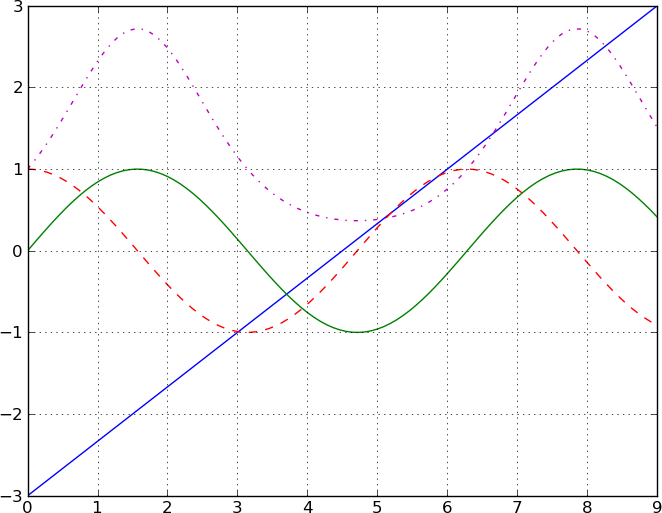
\includegraphics[scale=0.3]{img/plot3.png}
		\end{figure}
\end{frame}

% ------------------------------------------------------------------------------
\begin{frame}[t,fragile]{matplotlib}
	\begin{itemize}
		\item Controlando o estilo do plot
		\item A função plot aceita uma string especificando o estilo da linha
		e do símbolo usando o seguinte formato: '<color><linestyle><marker>'
	\end{itemize}
	
	\begin{tiny}
		
		\begin{table}
			\centering
			\begin{tabular}[r]{|cc||cc|}
				\hline
				\multicolumn{4}{|c|}{Cores (color)} \\
				\hline
				r & \textcolor{red}{vermelho} & c & \textcolor{cyan}{ciano} \\
				g & \textcolor{green}{verde}  & m & \textcolor{magenta}{magenta} \\
				b & \textcolor{blue}{azul}    & y & \textcolor{yellow}{amarelo} \\
				w & branco                    & k & preto \\
				\hline
			\end{tabular}
		\end{table}
		
		\vspace{-0.25cm}
		
		\begin{table}
			\centering
			\begin{tabular}[c]{|cc||cc||cc|}
				\hline
				\multicolumn{6}{|c|}{Símbolos (marker)} \\
				\hline
				. & pontos     & o & circulo       & \^{} & triangulo baixo \\
				s & quadrados  & + & cruz          & $v$ & triangulo cima  \\
				x & "xis"      & * & estrela       & $<$ & triangulo esq   \\
				D & diamante   & d & diamante peq. & $>$ & triangulo dir   \\
				\hline
			\end{tabular}
		\end{table}
		
		\vspace{-0.25cm}
		
		\begin{table}
			\centering
			\begin{tabular}[c]{|c||c|}
				\hline
				\multicolumn{2}{|c|}{Estilo da Linha (linestyle)} \\
				\hline
				-  & solid line    \\
				-- & dashed line   \\
				-. & dash-dot line \\
				:  & dotted line   \\
				\hline
			\end{tabular}
		\end{table}
	\end{tiny}
\end{frame}

% ------------------------------------------------------------------------------
\begin{frame}[t,fragile]{matplotlib}
		\begin{python}
		import numpy as np
		from pylab import *
		
		x = np.linspace(-6, 6, 500)
		plot(x,sin(x), label='sin(x)')
		>>> plot(x,cos(x), label='cos(x)')
		>>> title('Seno e Cosseno')
		>>> xlabel('x')
		>>> ylabel('f(x)')
		>>> axis([-6,6,-2,2])
		>>> legend(loc="upper right")
		\end{python}
		\begin{figure}
			\centering
			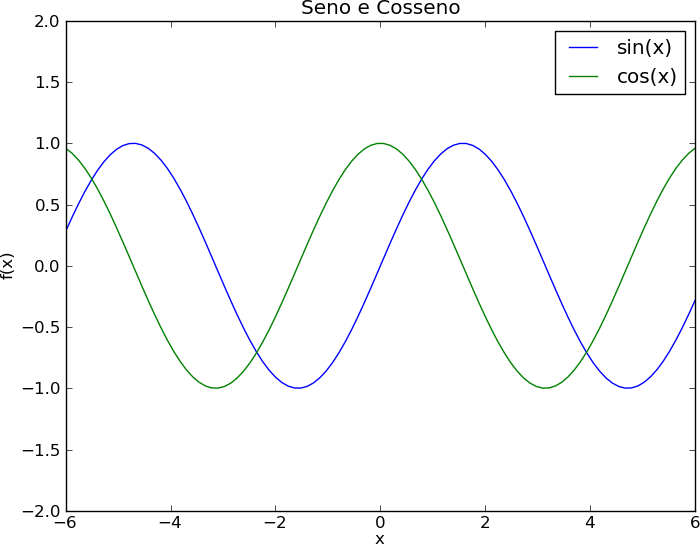
\includegraphics[scale=0.25]{img/plot4.png}
		\end{figure}	
\end{frame}

% ------------------------------------------------------------------------------
\begin{frame}[t,fragile]{matplotlib}
	\begin{itemize}
		\item Histogramas
		\item hist(x, bins=10)
		\item Distribuição normal $N(0,1)$
	\end{itemize}
	
	\begin{columns}
		\column{.55\textwidth}
		\begin{python}
>>> import numpy as np
>>> from pylab import *
>>> y = np.random.randn(1000)
>>> hist(y,bins=50)
		\end{python}
		
		\column{.5\textwidth}
		\vspace{-1cm}
		\begin{figure}
			\centering
			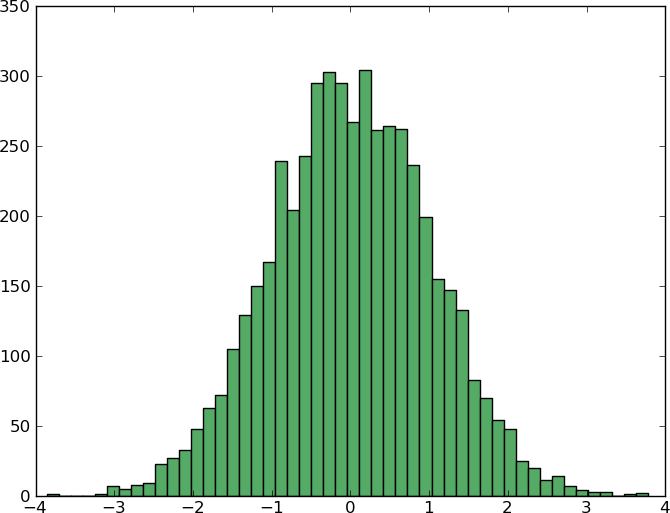
\includegraphics[scale=0.32]{img/plot5.png}
		\end{figure}
	\end{columns}
	
\end{frame}

% ------------------------------------------------------------------------------
\begin{frame}[t,fragile]{matplotlib}
	\begin{itemize}
		\item Gráfico de barras
		\item bar(x, height): plota um gráfico de barras com retângulos
		\item xticks(x, labels): posiciona rótulos dos retângulos
	\end{itemize}
	\begin{columns}
		\column{.6\textwidth}
		\begin{python}
>>> import numpy as np
>>> from pylab import *

>>> x=[1,2,3,4,5,6]
>>> y=[5,8,15,20,12,18]

>>> bar(x,y,align='center',
color='#2090AA')
>>> lab = ("D1","D2","D3","D4","D5","D6")
>>> xticks(x, lab)
		\end{python}
		
		\column{.4\textwidth}
		\begin{figure}
			\centering
			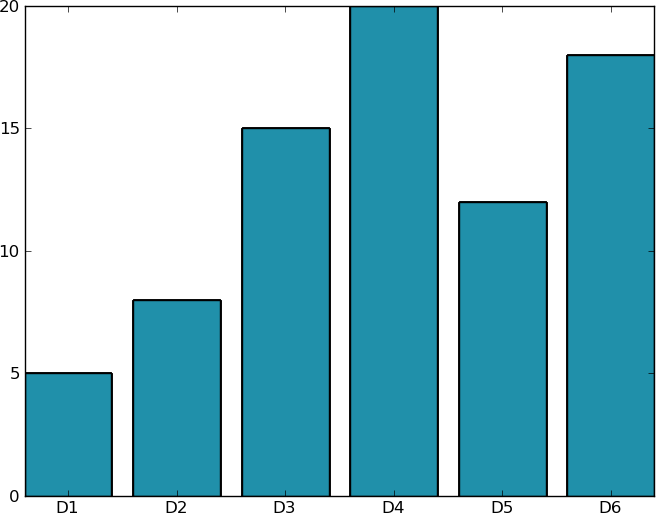
\includegraphics[scale=0.2]{img/plot6.png}
		\end{figure}
	\end{columns}
	
\end{frame}

% ------------------------------------------------------------------------------
\begin{frame}[t,fragile]{matplotlib}
	\begin{itemize}
		\item Salvando os gráficos em figuras
		\item savefig(filename):\\
		Salva a figura atual usando o formato.\\
		Alguns parâmetros opcionais:
		\begin{itemize}
			\item format: 'png', 'pdf', 'ps', 'eps', 'svg'
			\item transparent: True ou False
		\end{itemize}
	\end{itemize}
	\begin{python}
	>>> import numpy as np
	>>> from pylab import *
	>>> x = np.linspace(-3,3,1000)
	>>> y = sin(1/x)
	>>> plot(x,y)
	>>> savefig("seno1sx", format="eps")
	\end{python}
\end{frame}

% ------------------------------------------------------------------------------
\begin{frame}[t,fragile]{Galeria do matplotlib}
	\begin{figure}
		\centering
		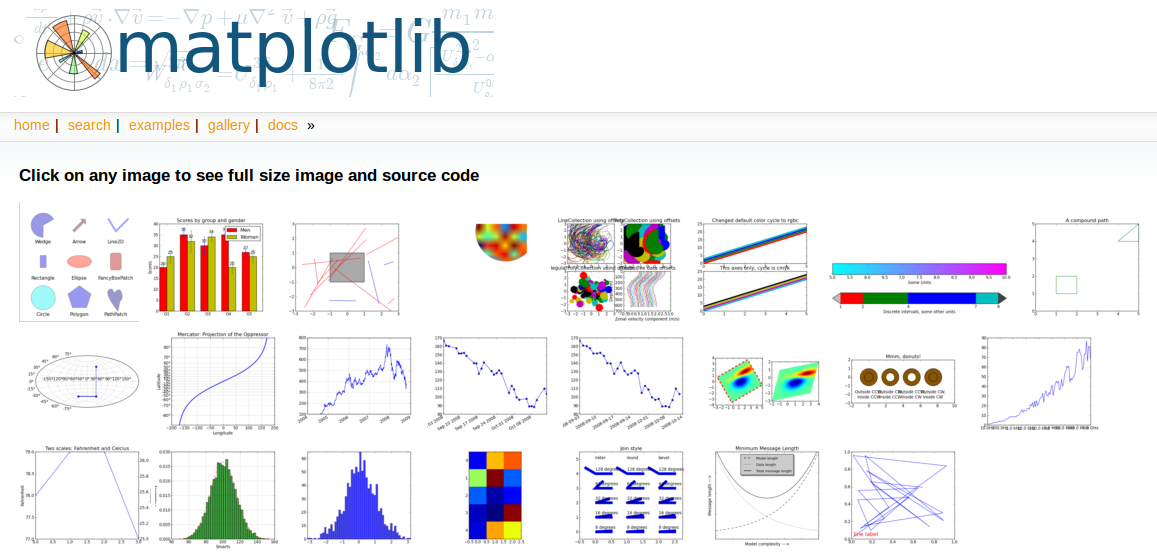
\includegraphics[scale=0.3]{img/matplot1.png}
	\end{figure}
\end{frame}

% ------------------------------------------------------------------------------
\begin{frame}[t,fragile]{Galeria do matplotlib}
	\begin{figure}
		\centering
		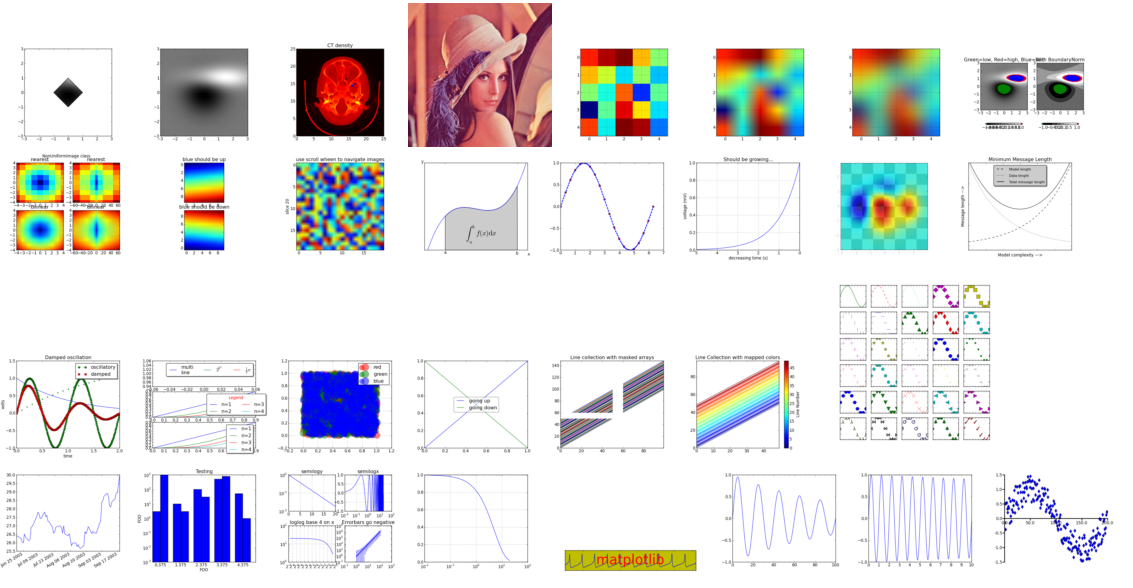
\includegraphics[scale=0.3]{img/matplot2.png}
	\end{figure}
\end{frame}

% ------------------------------------------------------------------------------
\begin{frame}[t,fragile]{Galeria do matplotlib}
	\begin{figure}
		\centering
		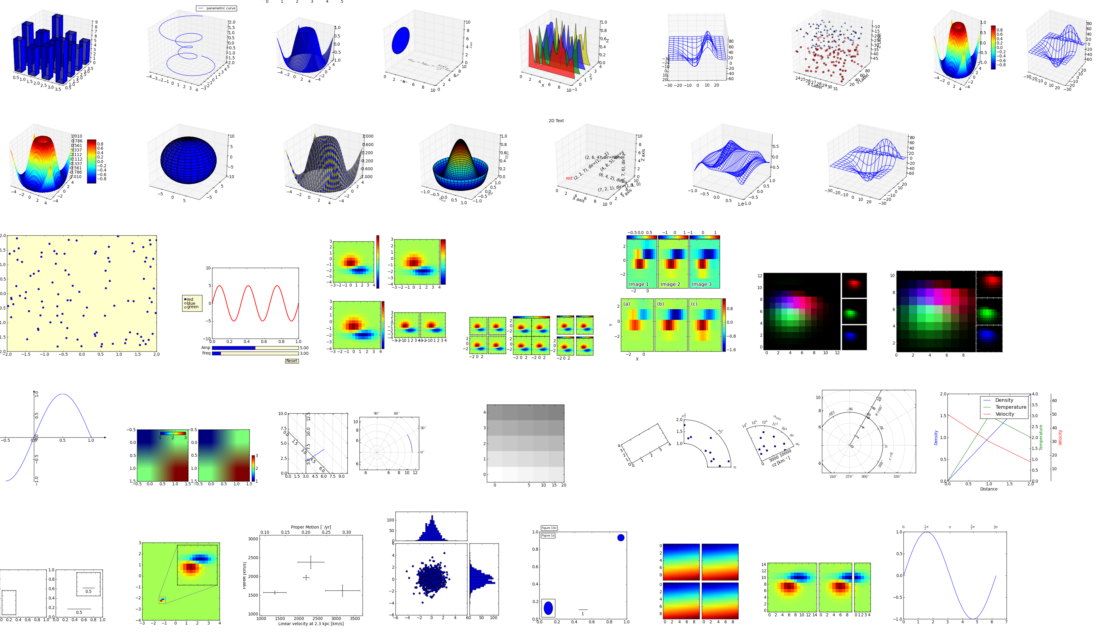
\includegraphics[scale=0.3]{img/matplot3.png}
	\end{figure}
\end{frame}

% ------------------------------------------------------------------------------
\begin{frame}[t,fragile]{Exemplo Completo}
	\begin{itemize}
		\item Problema: Resolver uma Equação Diferencial Ordinária (EDO)
		\item Encontrar $u(t)$ tal que
		$$u'(t) = f( u(t), t)$$
		\item dada a condição Inicial $$u(0) = u_0$$
		\item Exemplo: Crescimento exponencial (população) $$u'(t) = a u$$
		\item onde $a$ é uma constante dada que representa a taxa de crescimento de u.
	\end{itemize}
\end{frame}

% ------------------------------------------------------------------------------
\begin{frame}[t,fragile]{Exemplo Completo}
	\begin{itemize}
		\item Método de Euler Explícito
		$$u_{k+1} = u_k + \Delta t \ f(u_k, t_k)$$
		\item onde:
		\begin{itemize}
			\item $u_k$ é a aproximação numérica da solução exata $u(t)$ no tempo $t_k$
			\item $\Delta t$ é o passo de tempo
			\item $t_k = k \Delta t$, $k=0, \ldots, n$
		\end{itemize}
		\item Solução analítica para o exemplo $$u(t) = u_0 e^{a t}$$
	\end{itemize}
\end{frame}

% ------------------------------------------------------------------------------
\begin{frame}[t,fragile]{Exemplo Completo - Algoritmo}
	\begin{itemize}
		\item Dado: $u_0$, $a$, $T$, $\Delta t$
		\item Calcular $n$ (número de passos de tempo)
		\item Para k de 0 até n faça
		\begin{itemize}
			\item Calcular $u_{k+1}$ usando 
			$$u_{k+1} = u_k + f(u_k, t_k) \Delta t$$
		\end{itemize}
		\item Exibir os resultados
	\end{itemize}
\end{frame}

% ------------------------------------------------------------------------------
\begin{frame}[t,fragile]{Exemplo Completo - Python}
	\begin{itemize}
		\item $u'(t) = u, \quad u_0 = 1, \quad T = 3$
	\end{itemize}
	\begin{columns}
		\column{.4\textwidth}
		\begin{python}[]
import numpy as np
from pylab import *

u0 = 1
T  = 3.0
dt = 0.01
n  = int(T/dt)

# inicializa vetores
u = np.zeros(n+1)
v = np.zeros(n+1)
t = np.zeros(n+1)

# condicao inicial
t[0] = 0.0
u[0] = u0
\end{python}
\column{.6\textwidth}
\begin{python}[]
# loop no tempo
for k in range(n):
  u[k+1] = u[k] + dt * u[k]
  t[k+1] = t[k] + dt

# calcula solucao exata: 
# u(t) = u0 exp(at)
v = u0 * exp(t)

print v
print u

# exibe grafico da solucao
plot(t,v,color="r",
label="Solucao exata")
plot(t,u,
linestyle="--",color="b",
label="Solucao aproximada")
legend(loc="best")
show()    
		\end{python}
	\end{columns}
\end{frame}

% ------------------------------------------------------------------------------
\begin{frame}[t,fragile]{Exemplo Completo}
	\vspace{-0.5cm}
	\begin{figure}
		\centering
		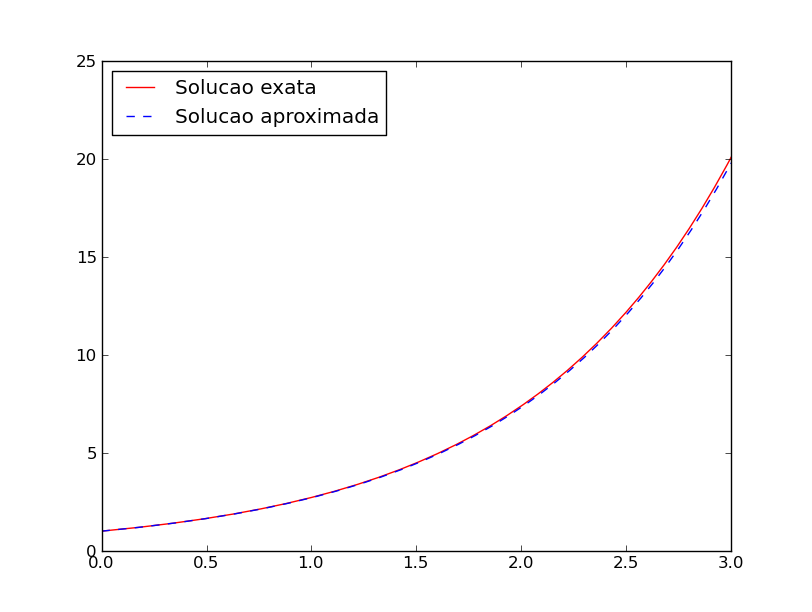
\includegraphics[scale=0.45]{img/euler.png}
	\end{figure}
\end{frame}

% ------------------------------------------------------------------------------
\begin{frame}[t,fragile]{Exemplo Completo com SciPy}
	\begin{itemize}
		\item scipy.integrate.odeint(func, y0, t)
		\item Usa a biblioteca \textbf{odepack} escrita em FORTRAN.
	\end{itemize}
	\begin{python}[]
from pylab import *
from scipy.integrate import odeint

def f(u,t):
  return u

T  = 3.0
u0 = 1.0
dt = 0.01
n  = int(T/dt)

t = np.linspace(0.0, T, n)
u = odeint(f,u0,t)

plot(t,u)
	\end{python}
\end{frame}

% ------------------------------------------------------------------------------

\begin{frame}
	\title{Parte IV}
	\subtitle{Outras bibliotecas e projetos com Python}
	\date{}\author{}\institute{}\date{}
	\maketitle
\end{frame}

% ------------------------------------------------------------------------------

\begin{frame}[t,fragile]{Sympy}
	\begin{figure}
		\centering
		
\includegraphics[scale=0.4]{img/sympylogo.png}
	\end{figure}
	\begin{itemize}
		\item Computação Simbólica
		\item Alternativa livre aos softwares Maple, Mathematica e Matlab.
		\item Aritmética básica, expansões, funções, derivadas, integrais, 
		substituições, limite, matrizes, etc.
	\end{itemize}
	\begin{columns}
		\column{.5\textwidth}
		\begin{python}
>>> from sympy import *
>>> x = Symbol('x')
>>> f = 2 * cos(x)
>>> diff(f, x)
-2*sin(x)
\end{python}
\column{.5\textwidth}
\begin{python}
>>> x = Symbol("x")
>>> limit(sin(x)/x, x, 0)
1
>>> limit(1/x, x, oo)
0
		\end{python}
	\end{columns}
\end{frame}

% ------------------------------------------------------------------------------
\begin{frame}[t]{Sage}
	\begin{figure}
		\centering
		
\includegraphics[scale=0.3]{img/logo_sage.png}
	\end{figure}
	\begin{itemize}
		\item Software matemático livre com liçenca GPL.
		\item Alternativa livre aos softwares Maple, Mathematica e Matlab.
		\item Re-utiliza pacotes como Maxima, GAP, Pari/GP, softwares de 
		renderização de imagens e outros.
		\item Disponível para uso online via browser.
	\end{itemize}
\end{frame}

% ------------------------------------------------------------------------------
\begin{frame}[t]{Visualização Científica}
	\begin{columns}
		\column{.5\textwidth}
		\begin{itemize}
			\item MayaVi
		\end{itemize}
		\begin{figure}
			\centering
			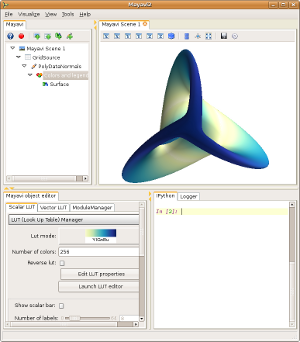
\includegraphics[scale=0.25]{img/mayavi-boy.png}
		\end{figure}
		\vspace{-0.5cm}
		\begin{figure}
			\centering
			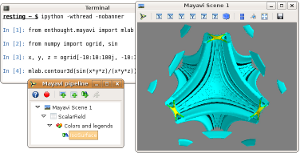
\includegraphics[scale=0.4]{img/mayavi-ipython.png}
		\end{figure}
		\column{.5\textwidth}
		\begin{figure}
			\centering
			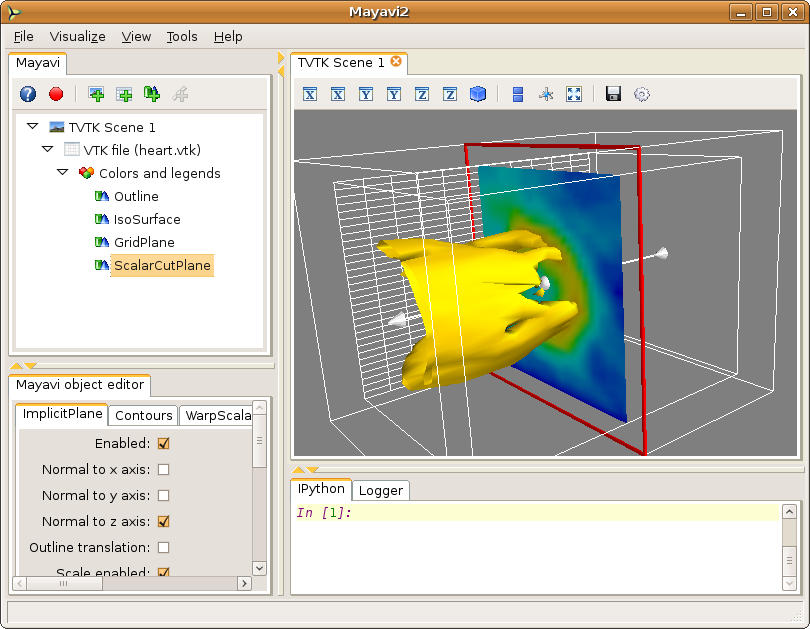
\includegraphics[scale=0.2]{img/heart.jpg}
		\end{figure}
	\end{columns}
\end{frame}

% ------------------------------------------------------------------------------
\begin{frame}[t]{Computação Gráfica, Visualização}
	\vspace{-0.5cm}
	\begin{columns}
		\column{.6\textwidth}
		%    \vspace{-0.5cm}
		\begin{figure}
			\centering
			
\includegraphics[scale=0.45]{img/vtk100.png}
		\end{figure}
		\vspace{-0.25cm}
		\begin{itemize}
			\item Computação gráfica, processamento de
			imagens e visualização.
			\item Escrito em C++ com interface em Tcl/Tk, Java e Python.
		\end{itemize}
		\vspace{-0.35cm}
		\begin{figure}
			\centering
			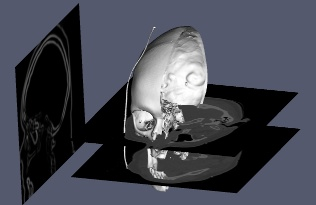
\includegraphics[scale=0.35]{img/vtk_ex.jpg}
		\end{figure}
		\column{.4\textwidth}
		\begin{figure}
			\centering
			
\includegraphics[scale=0.45]{img/opengl.jpg}
			\hspace{0.1cm}
			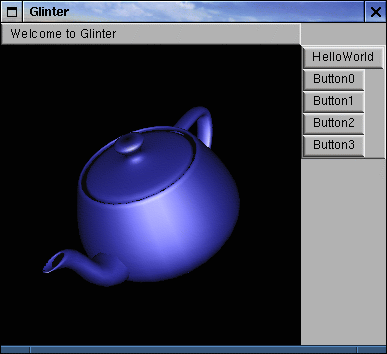
\includegraphics[scale=0.2]{img/pyogl.png}
		\end{figure}
		\begin{itemize}
			\item PyOpenGL: binding de OpenGL para Python
			\item OpenGL: API livre utilizada na computação gráfica
			\item Aplicativos gráficos, ambientes 3D, jogos.
		\end{itemize}
		
	\end{columns}
	
\end{frame}

% ------------------------------------------------------------------------------
\begin{frame}[t]{Álgebra Linear Computacional}
	\begin{columns}
		\column{.6\textwidth}
		\begin{figure}
			\centering
			
\includegraphics[scale=0.2]{img/pyamg.png}
		\end{figure}
		\begin{itemize}
			\item Algebraic Multigrid Solvers in Python
			\item Diversas implementações do AMG
			\item Fácil de usar, rápido, eficiente
			\item http://code.google.com/p/pyamg/
		\end{itemize}
		\column{.4\textwidth}
		\begin{figure}
			\centering
			
\includegraphics[scale=0.65]{img/logo_pysparse.png}
		\end{figure}
		\begin{itemize}
			\item PySparse: Biblioteca de matrizes esparsas
			\item Diversos formatos e métodos para conversão
			\item \textit{Solvers} iterativos (CG)
			\item Precondicionadores
		\end{itemize}
	\end{columns}
	
\end{frame}

% ------------------------------------------------------------------------------
\begin{frame}[t]{Solução Numérica de Equações Diferenciais}
	\begin{columns}
		\column{.5\textwidth}
		\vspace{-0.7cm}
		\begin{figure}
			\centering
			
\includegraphics[scale=0.3]{img/fenics.png}
		\end{figure}
		\begin{itemize}
			\item FEniCS Project
			\item Solução automatizada de EDPs usando o método dos elementos finitos
			\item Alto nível de abstração (Muito próximo da formulação matemática)
			\item Paralelismo, adaptatividade, estimativa de erro, etc
		\end{itemize}
		\column{.5\textwidth}
		\vspace{-0.75cm}
		\begin{figure}
			\centering
			
\includegraphics[scale=0.65]{img/logo_fipy.png}
		\end{figure}
		\begin{itemize}
			\item FiPy (A finite volume PDE solver written in Python)
			\item Solver de EDPs usando o método dos volumes finitos
			\item Orientado a objetos
			\item Computação paralela
		\end{itemize}
	\end{columns}
	
\end{frame}

% ------------------------------------------------------------------------------
\begin{frame}[t]{Apredizagem de Máquina}
	\begin{columns}
		\column{.5\textwidth}
		\vspace{-0.5cm}
		\begin{figure}
			\centering
			
\includegraphics[scale=0.25]{img/shogun_logo.png}
		\end{figure}
		\begin{itemize}
			\item Shogun: A Large Scale Machine Learning Toolbox
			\item SVM (Support Vector Machines)
			\item http://www.shogun-toolbox.org/
		\end{itemize}
		\column{.5\textwidth}
		\vspace{-1.25cm}
		\begin{figure}
			\centering
			
\includegraphics[scale=0.4]{img/logo_scikit-learn.png}
		\end{figure}
		\begin{itemize}
			\item Construído sobre NumPy, SciPy e Matplotlib
			\item Diversas técnicas como p. ex. SVM, K-Means, etc
			\item http://scikit-learn.sourceforge.net
		\end{itemize}
	\end{columns}
	
\end{frame}

% ------------------------------------------------------------------------------
\begin{frame}[t]{Python para Física}
	\begin{itemize}
		\item Astropysics: http://packages.python.org/Astropysics/
		\begin{itemize}
			\item Utilitários de astrofísica em Python
		\end{itemize}
		\item PyFITS: http://packages.python.org/pyfits/
		\begin{itemize}
			\item Manipulação de imagens FITS em Python
		\end{itemize}
		\item YT: http://yt-project.org/
		\begin{itemize}
			\item yt é um toolkit para manipular dados de simulações astrofísicas
			com suporte para análise e visualização.
		\end{itemize}
	\end{itemize}
	
	\begin{figure}
		\centering
		
\includegraphics[scale=1.0]{img/astropysics.png}
		\hspace{0.25cm}
		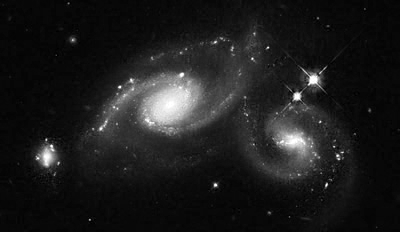
\includegraphics[scale=0.2]{img/pyfits-ex.jpg}
		\hspace{0.25cm}
		
\includegraphics[scale=0.4]{img/yt_icon.png}
	\end{figure}
\end{frame}

% ------------------------------------------------------------------------------
\begin{frame}[t]{Python para Química}
	\begin{itemize}
		\item Cheminformatics: OpenBabel (Pybel), RDKit, OEChem, Daylight 
		(PyDaylight), Cambios Molecular Toolkit, Frowns, PyBabel and MolKit 
		\item Computational chemistry: OpenBabel, cclib, QMForge, GaussSum, 
		PyQuante, NWChem, Maestro/Jaguar, MMTK
		\item Visualisation: CCP1GUI, PyMOL, PMV, Zeobuilder, Chimera, VMD
	\end{itemize}
	
	\begin{figure}
		\centering
		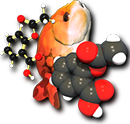
\includegraphics[scale=0.5]{img/babel130.png}
	\end{figure}
\end{frame}

% ------------------------------------------------------------------------------

\begin{frame}
	\frametitle{The zen of Python}
	\begin{center}
		\begin{scriptsize}
			Beautiful is better than ugly.\\
			Explicit is better than implicit.\\
			Simple is better than complex.\\
			Complex is better than complicated.\\
			Flat is better than nested.\\
			Sparse is better than dense.\\
			Readability counts.\\
			Special cases aren’t special enough to break the rules.\\
			Although practicality beats purity.\\
			Errors should never pass silently.\\
			Unless explicitly silenced.\\
			In the face of ambiguity, refuse the temptation to guess.\\
			There should be one- and preferably only one -obvious way to do it.\\
			Although that way may not be obvious at first unless you’re Dutch.\\
			Now is better than never.\\
			Although never is often better than *right* now.\\
			If the implementation is hard to explain, it’s a bad idea.\\
			If the implementation is easy to explain, it may be a good idea.\\
			Namespaces are one honking great idea - let’s do more of those!\\
		\end{scriptsize}
	\end{center}
\end{frame}

% ------------------------------------------------------------------------------
\begin{frame}[t]{Referências}
	\vspace{-1cm}
	\begin{columns}
		\column{.75\textwidth}
		\begin{itemize}
			\item Hans Petter Langtangen - "A Primer on Scientific Computing
			with Python"
			\item Hans Petter Langtangen - "Python Scripting"
			\item Mark Lutz - "Learning Python"
			\item Slides de Rafael Sachetto Oliveira (UFSJ)
			\item Slides de Felix Steffenhagen (Uni Freiburg)
			\item Mais informações:
			\begin{itemize}
				\item http://www.python.org
				\item http://numpy.org
				\item http://ark4n.wordpress.com/python/
				\item http://fperez.org/py4science/
			\end{itemize}
			\item Equipe da Semana da Computação/Prof. Rafael Sachetto
		\end{itemize}
		\column{.25\textwidth}
		\begin{figure}
			\centering
			\includegraphics[scale=0.15]{img/book.png}
			\\
			\includegraphics[scale=0.25]{img/pypd.jpg}
		\end{figure}
	\end{columns}
\end{frame}

% ------------------------------------------------------------------------------

\begin{frame}
  \frametitle{Pós-Graduação em Modelagem Computacional}
  \begin{center}
  \bi
  \item UFJF
  \item Mestrado e Doutorado
  \item \textbf{www.ufjf.br/pgmc}
  \ei
  \begin{figure}
    \centering
    \includegraphics[scale=0.25]{img/pgmc.png}
  \end{figure}
  \end{center}
\end{frame}

% ------------------------------------------------------------------------------
\begin{frame}[t]{Agradecimentos}
	\bi
	\item Prof. Rafael Sachetto Oliveira
	\item Prof. Bernardo Martins Rocha
	\item Prof. Ruy Freitas Reis
	\item Profa. Bárbara de Melo Quintela
	\item Prof. Igor de Oliveira Knop
	\item Equipe da Semana da Computação
	\item Departamento de Ciência da Computação - UFSJ
	\item Departamento de Ciência da Computação - UFJF
	\ei
\end{frame}

% ------------------------------------------------------------------------------

\begin{frame}
	\title{Fim}
	\date{}\author{}\subtitle{}\institute{}\date{}
	\maketitle
\end{frame}

% ------------------------------------------------------------------------------

\end{document}

% ------------------------------------------------------------------------------
